\documentclass[times, utf8, diplomski]{fer}

\usepackage{booktabs}
\usepackage{float}
\usepackage{algpseudocode}
\usepackage{algorithm}
\usepackage{pdfpages}
\usepackage{hyperref}

\algnewcommand\OrWord{\textbf{ or }}
\algnewcommand\AndWord{\textbf{ and }}

\algnewcommand\algorithmicforeach{\textbf{for each}}
\algdef{S}[FOR]{ForEach}[1]{\algorithmicforeach\ #1\ \algorithmicdo}

\newcommand{\classname}[1]{\texttt{#1}}

\graphicspath
{
	{./images/}
	{./images/Transport/}
	{./images/HLAPI/}
	{./images/Application/}
}

\setcitestyle{numbers}
\setcitestyle{square}

\begin{document}

\thesisnumber{2963}
\title{Razvoj i primjena biblioteke za umrežavanje višekorisničkih videoigara}
\author{Filip Nemec}

\maketitleeng
\maketitle

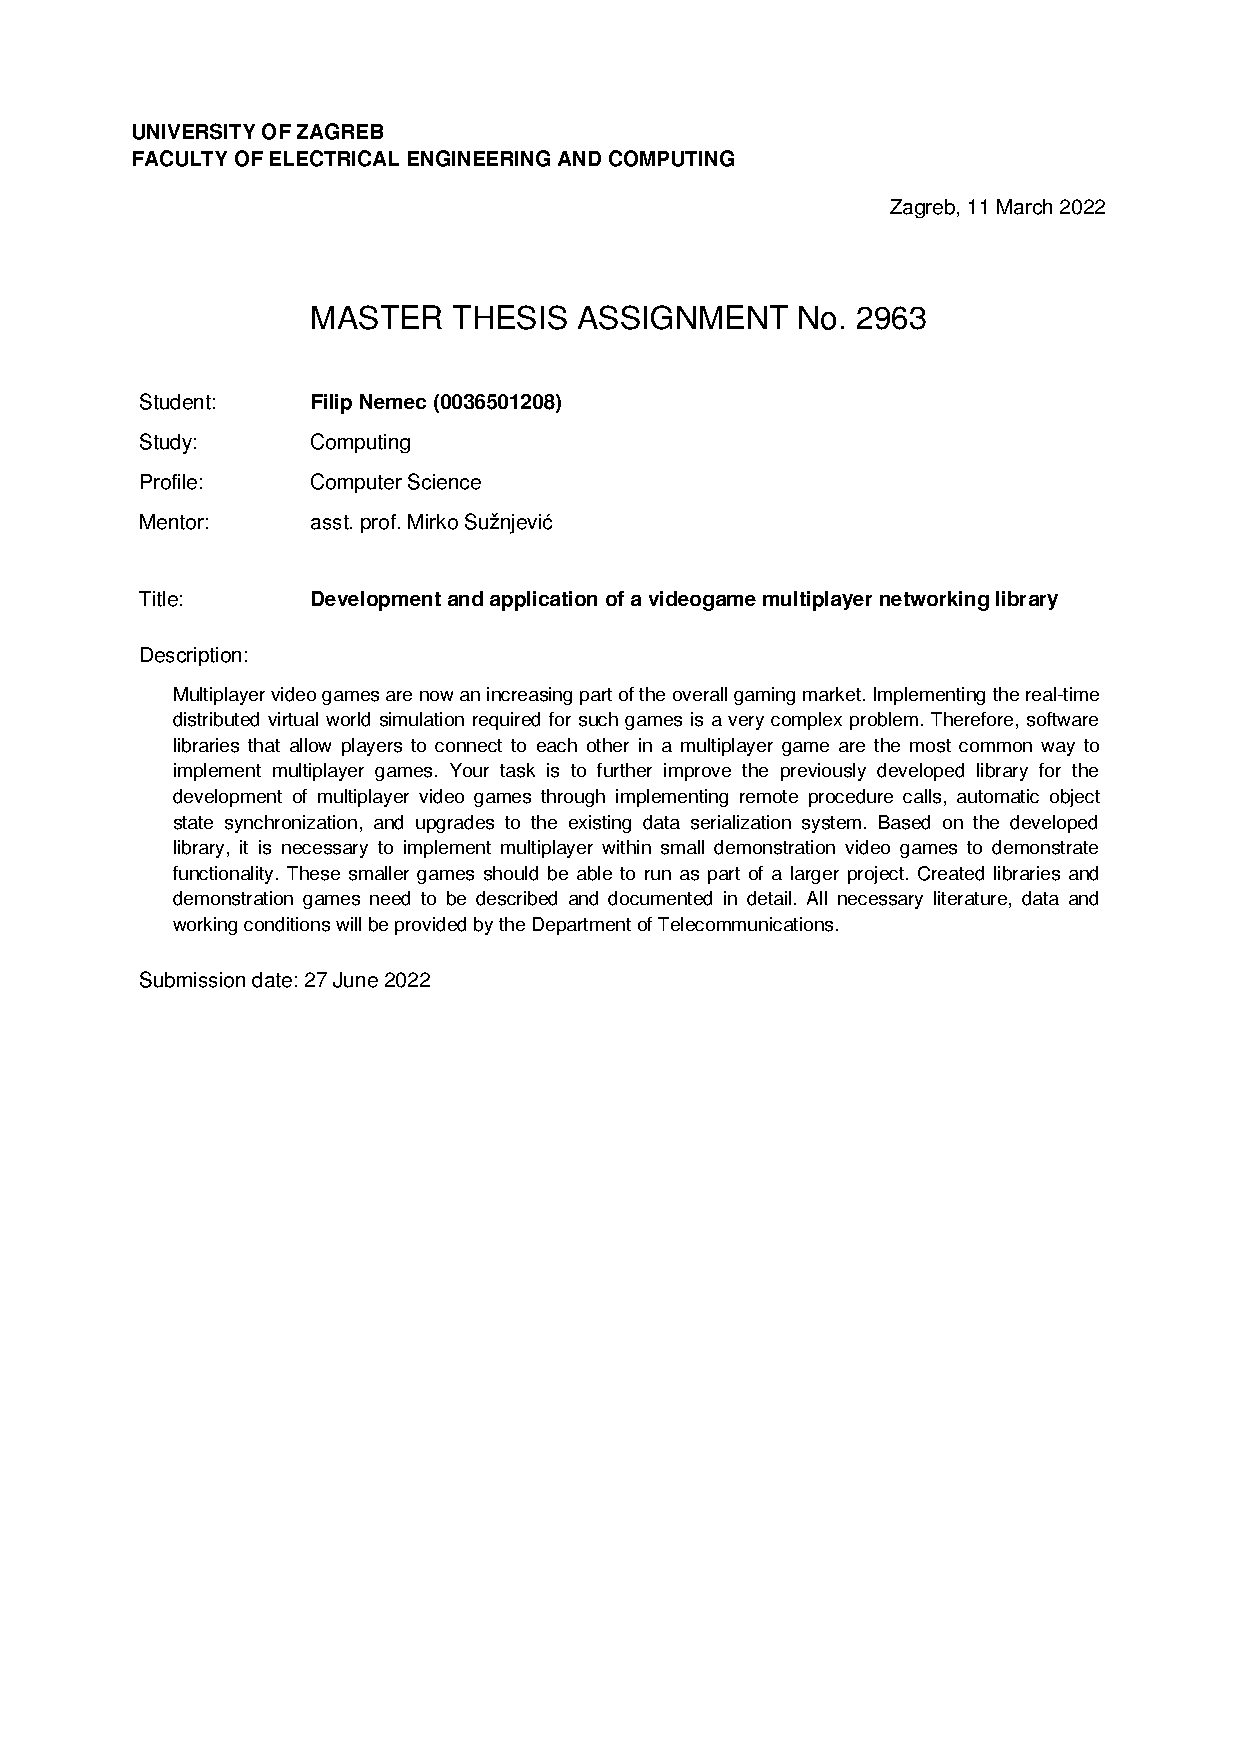
\includepdf[pages=-]{task.pdf}

% Ispis stranice s napomenom o umetanju izvornika rada. Uklonite naredbu \izvornik ako želite izbaciti tu stranicu.
% \izvornik

% Dodavanje zahvale ili prazne stranice. Ako ne želite dodati zahvalu, naredbu ostavite radi prazne stranice.
% \zahvala{}

{\footnotesize\tableofcontents}

\chapter{Introduction}
In the recent years, multiplayer\footnote{https://en.wikipedia.org/wiki/Multiplayer\_video\_game} games have been on the rise. There are many reasons for it, with main ones being social interactions, replayability and unique experiences they provide. For a game to be considered multiplayer, it has to support a way for multiple human players to experience and participate in the game. Based on that simple requirement, games can implement multiplayer in a variety of ways:

\begin{enumerate}
	\item \textbf{Local multiplayer} in which the game runs on a single computing system. Popular implementations of local multiplayer include \textit{shared screen} and \textit{split screen}. In shared screen games, all players see the game from a single camera perspective, while in split screen mode each player has its portion of the screen which shows the game from an individual player's perspective. In terms of implementation difficulty, this is the simplest form of multiplayer and is not much different from single-player.
	
	\item \textbf{LAN multiplayer} in which the game runs on multiple computing systems and game simulation is synchronized over a local area network\footnote{https://en.wikipedia.org/wiki/Local\_area\_network}. Since local area networks are usually extremely fast and reliable, multiplayer implementation does not cause many problems.
	
	\item \textbf{WAN multiplayer} is similar to LAN, except game simulation is synchronized over a wide area network\footnote{https://en.wikipedia.org/wiki/Wide\_area\_network} such as the Internet. Multiplayer over wide area networks requires the most complex implementation considering the unreliability and latency of such networks.
\end{enumerate}

\begin{figure}[H]
	\centering
	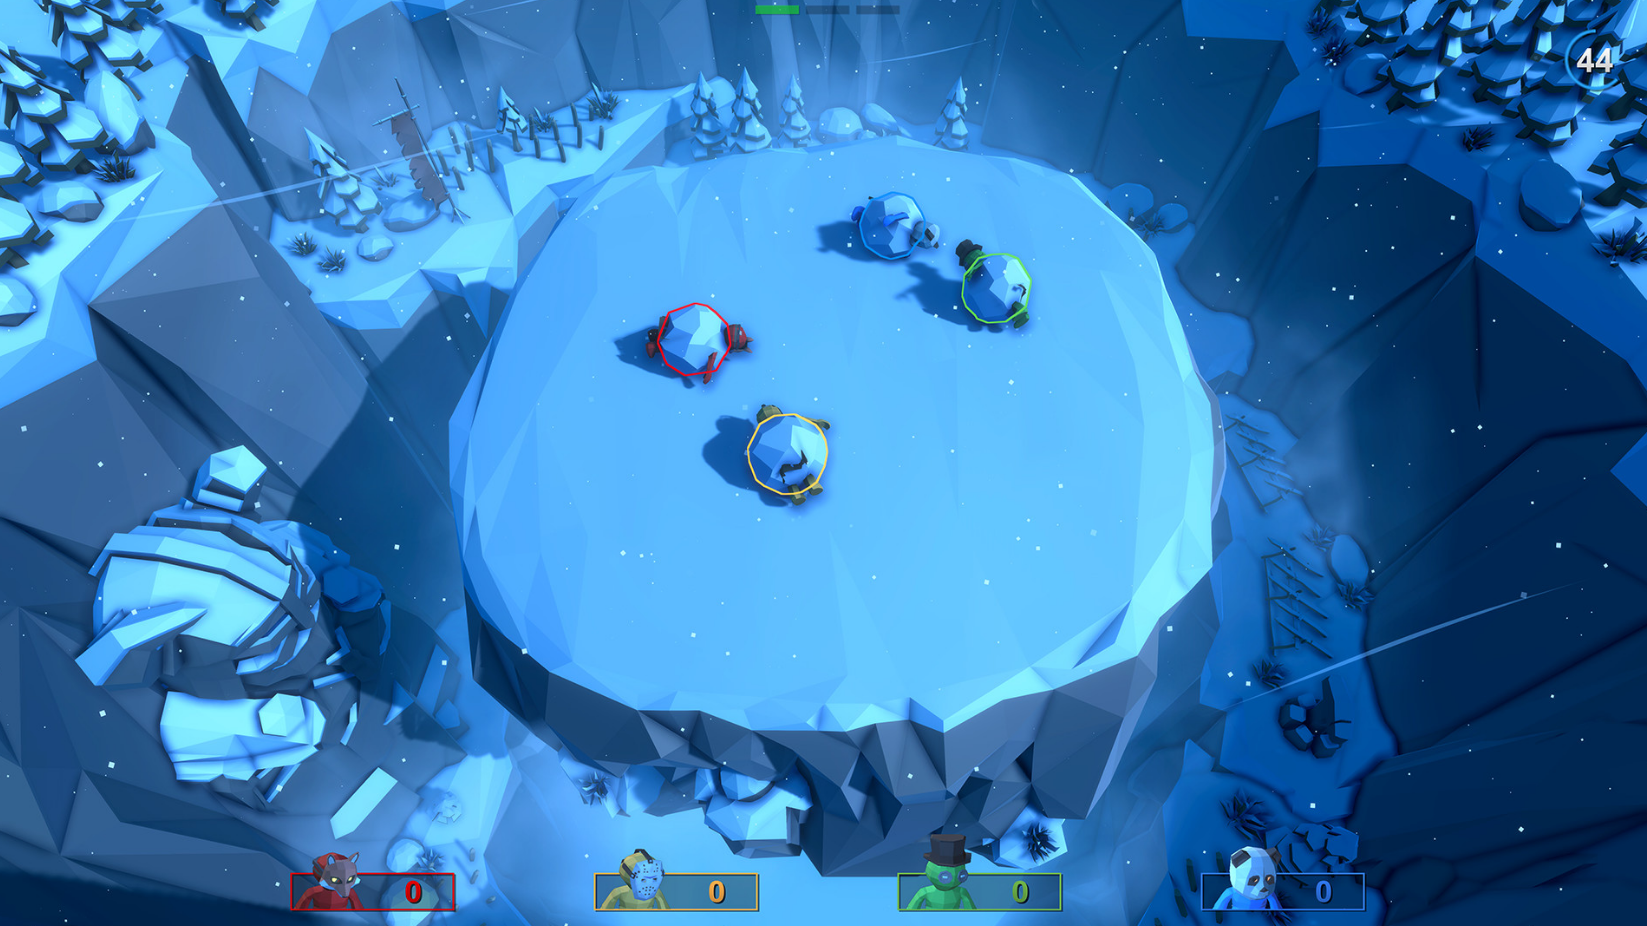
\includegraphics[scale=0.66]{Pummel-Party}
	\caption{\textit{Pummel Party}, example of a multiplayer game.}
	\label{fig:pummel}
\end{figure}
 
Development of video-games is a process which requires a wide variety of skills. Adding the requirement of multiplayer functionality to such a process greatly increases the complexity and development time required for creating the final game. For that reason, game developers rarely directly implement multiplayer solutions, but rather use existing networking libraries that provide high-level features for easy prototyping and fast development cycles. This thesis explains how such a solution can be implemented from the ground up and then used to create a simple multiplayer game, such as \ref{fig:pummel}. \\

\chapter{Transport}
This chapter introduces and explains in detail the concept of a transport layer. It starts by giving an introduction to networking, explaining motivation behind a layered structure. It then discusses today's most widely used transport layers. Finally, it finishes by giving a detailed look into a custom transport layer implementation.

\section{Introduction}
Computer networking is a complex problem that consists of many different sub-problems, such as packet-routing, data transmission, integrity, reliability, congestion-control, flow-control and much more. To deal with such complexity, ISO (International Organization for Standardization)\footnote{https://en.wikipedia.org/wiki/International\_Organization\_for\_Standardization} developed OSI (Open Systems Interconnection) model\footnote{https://en.wikipedia.org/wiki/OSI\_model} in the year 1984. OSI model divides the complex problem of computer networking into a structure consisting of 7 layers\footnote{https://www.geeksforgeeks.org/layers-of-osi-model/} (which can be seen at \ref{fig:osi-layers}), each layer building on top of the layer below it. Layers are defined as follows:

\begin{enumerate}
	\item \textbf{Physical layer} is responsible for transmission of raw signals between two or more physical entities. Jobs of this layer include transmission of bits, bit-rate control and support for various modes of transmission such as simplex, half-duplex and full-duplex\footnote{https://www.geeksforgeeks.org/transmission-modes-computer-networks/}.
	
	\item \textbf{Data-link layer} enables communication between two neighboring network nodes (devices). Basic functions of this layer include point-to-point frame transmission, error-control and data-flow control. 
	
	\item \textbf{Network layer} solves the problem of end-to-end device communication. Functions of network layer include routing (finding optimal route for data to reach its destination) and logical addressing (ability to uniquely identify a device on the computer network).
	
	\item \textbf{Transport layer} is responsible for transmission of data from process-to-process while satisfying a transparency criterion. There are two types of transparencies \cite{kommre}:
	
	\begin{enumerate}
		\item \textit{Semantic transparency} whose only task it to ensure that data arrives reliably and in-order it was sent.
		\item \textit{Temporal transparency} that only focuses on delivering data as fast as possible.
	\end{enumerate}

	\item \textbf{Session layer} is responsible for establishing, maintaining and terminating connections between hosts, authentication and security.
	
	\item \textbf{Presentation layer} is responsible for encryption/decryption, compression and translation between data formats.
	
	\item \textbf{Application layer} is responsible for producing, processing and displaying data to the end-user.
\end{enumerate}

With such layered structure, \textit{abstraction} was introduced. Every layer simply uses implementation below it without the need to know how it is implemented. This gives engineers the ability to easily swap out implementations of different layers in the stack.


\begin{figure}[h!]
	\centering
	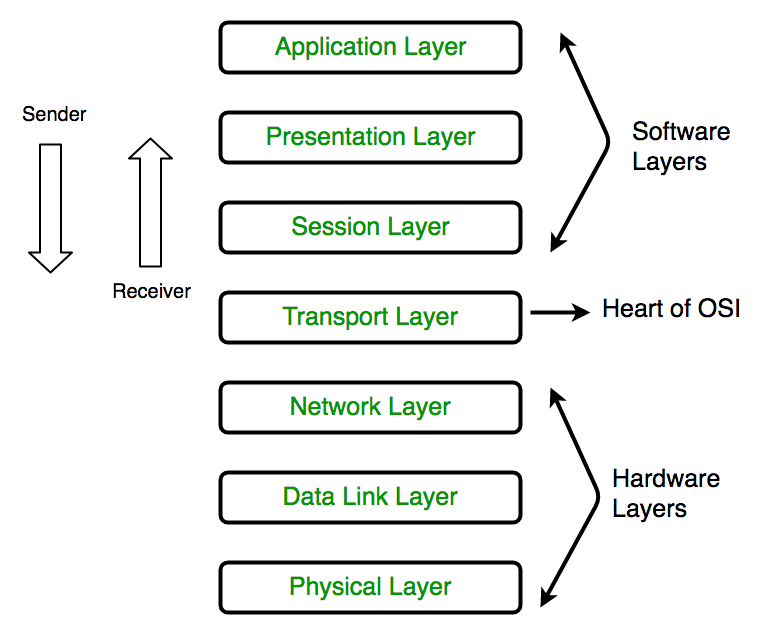
\includegraphics[scale=0.34]{OSI-model-layers}
	\caption{OSI layers, from \cite{GeeksForGeeks:OSI-model}}
	\label{fig:osi-layers}
\end{figure}


\section{Existing transport implementations}
Previous section mentioned the terms of semantic and temporal transparency. Consequently, there exist two different transport layer implementations, one for each transparency type. \\

The first protocol, which implements semantic transparency, is called \textit{Transmission Control Protocol}\footnote{https://datatracker.ietf.org/doc/html/rfc793} (left column at \ref{fig:tcp-vs-udp}). TCP abstracts away the concept of computer network and exposes a simple interface to the user, where writing bytes over the network is indistinguishable from writing to a simple binary file. TCP implements many complex features to ensure data arrives complete and in-order. It also enforces congestion control, where TCP dynamically adjusts send rate in order to not congest the network. \\

The second protocol, which implements temporal transparency, is called \textit{User Datagram Protocol}\footnote{https://datatracker.ietf.org/doc/html/rfc768} (right column at \ref{fig:tcp-vs-udp}). UDP is a protocol that implements a thin layer of abstraction over the network layer. UDP does not add any complex features that TCP has, it simply adds four more fields to the packet: source port, destination port, length and checksum. Its simplicity results in higher performance, but at the cost of reliability and order: packets can be lost or duplicated in transit and order of packets is not guaranteed.\\

\begin{figure}[H]
	\centering
	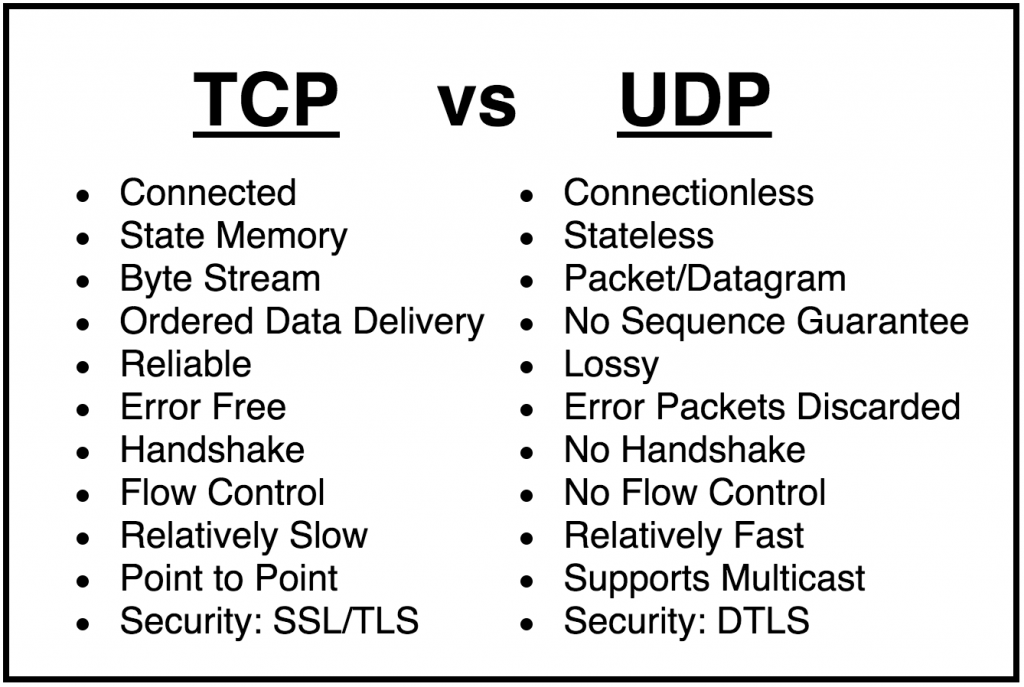
\includegraphics[scale=0.35]{TCP-vs-UDP}
	\caption{Comparison between TCP and UDP protocols, from \cite{NetBurner:TCP-vs-UDP}}
	\label{fig:tcp-vs-udp}
\end{figure}


\section{Custom transport implementation}
While TCP and UDP are successful at solving most use-cases, there exists a major limitation: each protocol solves only one type of transparency. At the time those protocols were developed, it was thought those protocols could be used for solving all the problems. \\

However, with the rise of online gaming, the need for having both transparency implementations at once appeared; some data would require reliability and ordering that TCP provides (for example, textual chat messages), while other types needed only latest data without the guarantee of delivery (for example, position of the player in a virtual world). \\

Using both protocols at the same time, based on the type of data, is not an ideal solution either, for multiple reasons \cite{GafferOnGames:UDP-vs-TCP}:

\begin{enumerate}
	\item Using TCP can induce packet loss in UDP packets as routers often prioritize TCP segments (as dropping TCP segment requires re-sending, while dropping UDP packet does not).
	\item Supporting many reliable channels (for example, one channel for text message data, another for images or audio) would require many TCP connections, quickly exhausting operating system resources.
	\item Application code-base would be hard to manage, potentially resulting in slower development and harder to track bugs.
\end{enumerate}

For all of those reasons, a custom solution is required - one that allows the user to easily specify, on per packet basis, how data should be delivered. If data is time-sensitive, user must be able to send it in unreliable manner, preserving temporal transparency. If data is important and must be delivered, semantic transparency must be preserved. As UDP already provides temporal transparency, it simply needs to be upgraded it with \textbf{optional} semantic transparency features that are present in the TCP. Implementations of such protocols are often called RUDP - \textit{Reliable User Datagram Protocol}. The rest of this chapter explains one such implementation.



\subsection{Packet}
\classname{Packet} represents a single outgoing message of arbitrary data that can be sent over the network. It is a thin abstraction layer over raw byte-array and therefore offers benefits that a raw byte-array cannot. \\

One such benefit is object pooling\footnote{https://en.wikipedia.org/wiki/Object\_pool\_pattern}. As creation of packets is a very frequent occurrence in networked applications, allocating new packet instances each time a packet is needed would quickly fill-up heap memory, prompting execution of garbage collection\footnote{https://en.wikipedia.org/wiki/Garbage\_collection\_(computer\_science)}. This is especially important in applications that have time constraints, such as games, where even one slowly executed frame could ruin user experience. \\

Another benefit is separation of write-only and read-only operations. Since \classname{Packet} represents an outgoing packet, it only offers methods for writing data (constructing the packet). Those methods also provide powerful functionality, allowing user to construct packets containing complex structures, as demonstrated by \ref{fig:packet-write}. \\

\begin{figure}[h!]
	\centering
	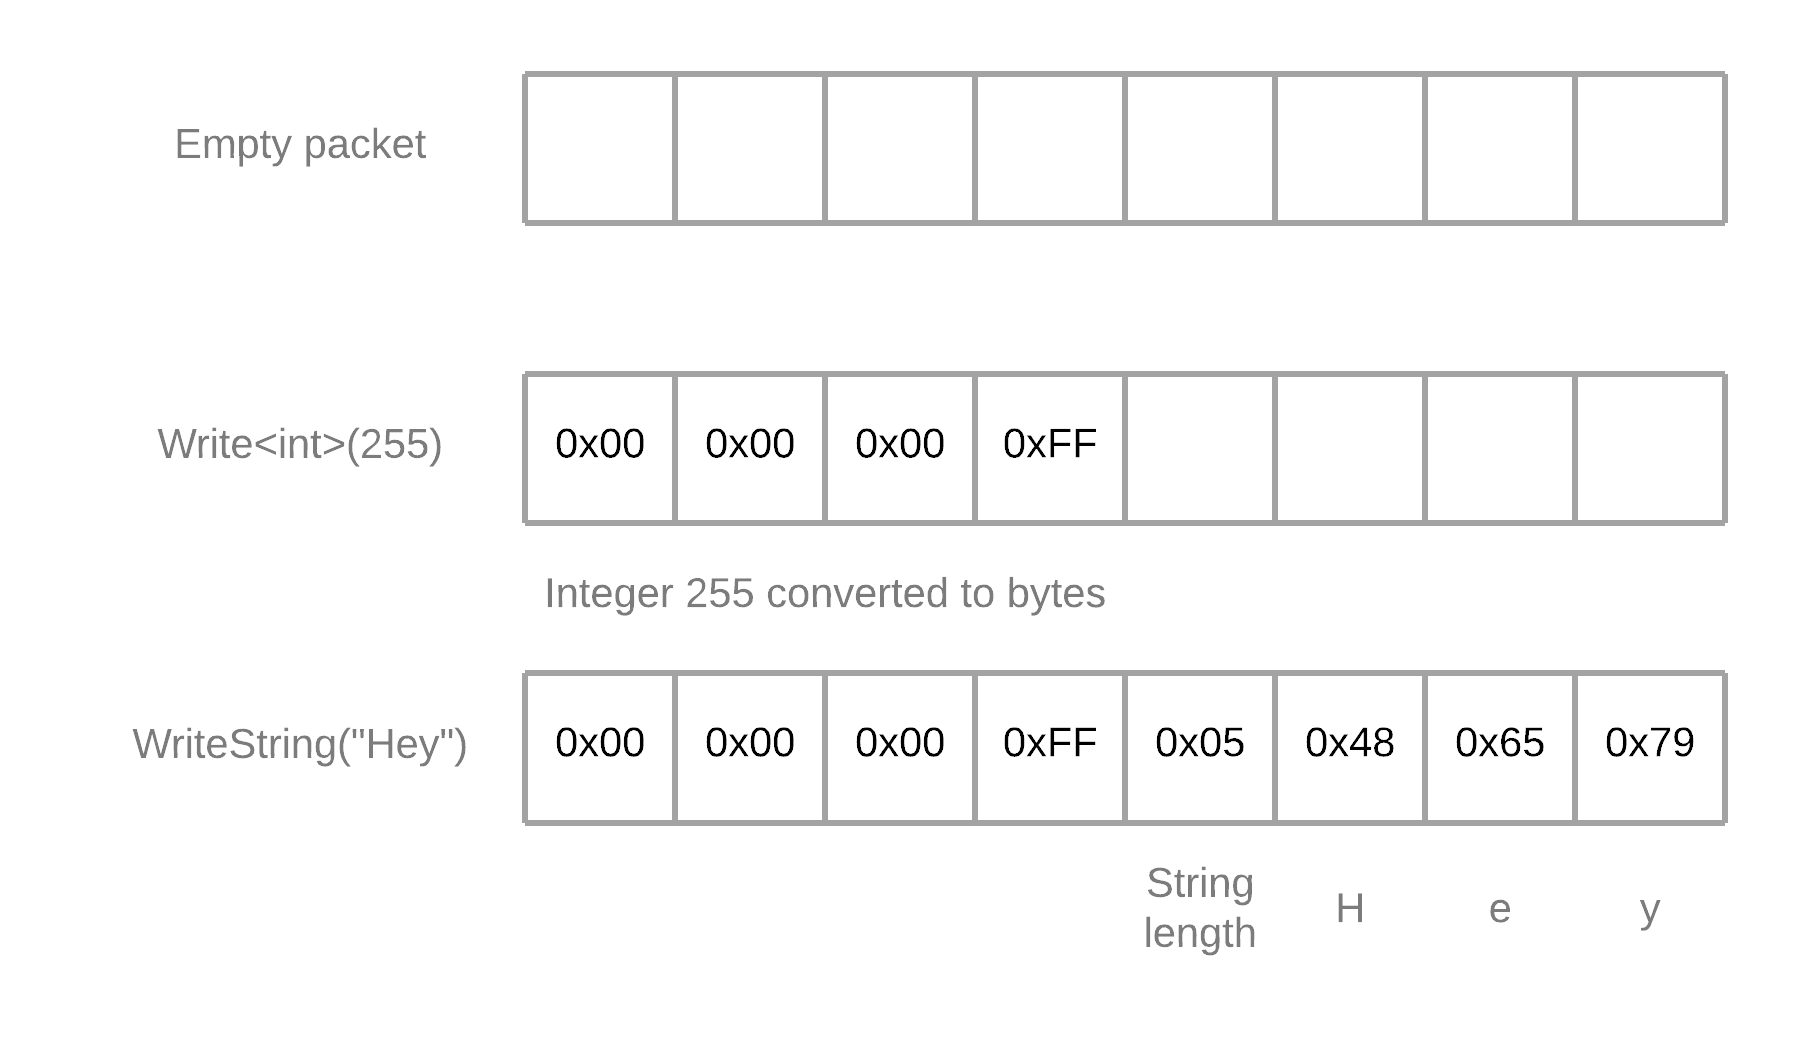
\includegraphics[scale=0.22]{Packet-write}
	\caption{Example of writing data to a packet}
	\label{fig:packet-write}
\end{figure}

Similarly to \classname{Packet}, which is write-only, \classname{Read\-Only\-Packet} is a read-only view that represents a single incoming message of arbitrary data that was received over the network. It offers the same interface as \classname{Packet}, but instead of write, read methods are exposed. Another important feature of \classname{Read\-Only\-Packet} is that it cannot in any way modify underlying packet data, making it very safe to use, even in multi-threaded scenarios. \\

Finally, the last benefit is cleaner code. Spotting an instance of \classname{Packet} or \classname{Read\-Only\-Packet} immediately gives information to the reader that this code works with networking. Same could not be said for byte-array as its usages are much broader. \\

\classname{Packet} also defines an important constant, which is the maximum size, in bytes. This constant was carefully chosen to avoid packet fragmentation on the network layer. Any packets that require bigger size must use a fragmented channel which will perform fragmentation and reassembly on the application layer. Maximum size is equal to Ethernet MTU (Maximum transmission unit, 1500 bytes) subtracted by IP header size (20 bytes) and UDP header size (8 bytes), which results in maximum size of 1472 bytes.\\

\begin{equation}
	Maximum \; size = 1500 - 20 - 8 = 1472 \; bytes \label{eq:max_packet_size}
\end{equation}

\subsubsection{Packet structure}
Each packet follows the same structure, which is a header type followed by the header-specific payload (\ref{fig:packet-structure}). It is important to mention that header is always inserted as the first byte without any exceptions.

\begin{figure}[h!]
	\centering
	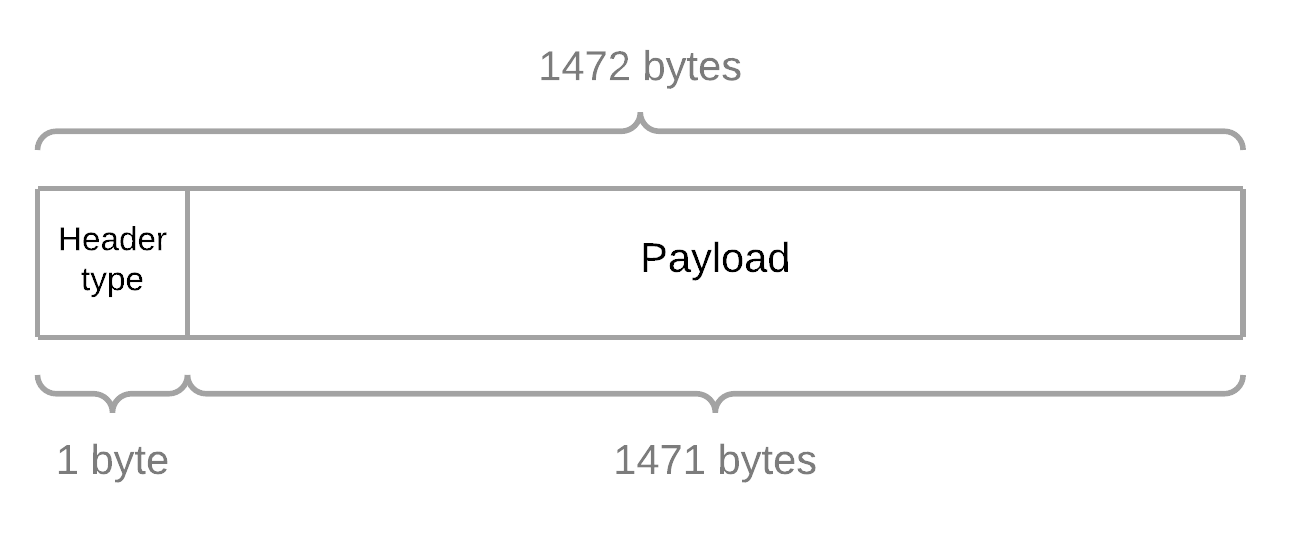
\includegraphics[scale=0.25]{Packet-structure}
	\caption{Packet structure}
	\label{fig:packet-structure}
\end{figure}


\subsubsection{Header types}
Header type is used to denote what kind of packet it is and allows the receiver to decode the meaning behind received bytes.

\begin{table}[H]
	\centering
	\resizebox{\textwidth}{!}{%
		\begin{tabular}{|c|c|c|}
			\hline
			\textbf{Header type} & \textbf{Description}                                                                                                                   & \textbf{Payload}                                                                       \\ \hline
			Connect              & \begin{tabular}[c]{@{}c@{}}Sent by the client to server when\\ establishing a virtual connection.\end{tabular}                         & Optional connect data                                                                  \\ \hline
			ConnectApproved      & \begin{tabular}[c]{@{}c@{}}Sent by the server to client when\\ connection request has been approved.\end{tabular}                      & -                                                                                      \\ \hline
			Ping                 & \begin{tabular}[c]{@{}c@{}}Used for measuring connection latency\\ and serves as a keep-alive packet.\end{tabular}                     & Sequence number                                                                        \\ \hline
			Pong                 & Response to the ping packet.                                                                                                           & Sequence number                                                                        \\ \hline
			Data                 & Indicates that the packet contains data.                                                                                               & \begin{tabular}[c]{@{}c@{}}Channel ID, channel header,\\ application data\end{tabular} \\ \hline
			Acknowledgement      & \begin{tabular}[c]{@{}c@{}}Indicates that specific set of\\ packets have been received.\end{tabular}                                   & \begin{tabular}[c]{@{}c@{}}Channel ID, sequence number,\\ ack bit-field\end{tabular}   \\ \hline
			Disconnect           & \begin{tabular}[c]{@{}c@{}}Sender has closed its side of the connection and\\ will no longer send or receive any packets.\end{tabular} & -                                                                                      \\ \hline
			Timeout              & Indicates that a connection has timed-out.                                                                                             & -                                                                                      \\ \hline
		\end{tabular}%
	}

	\caption{All of the possible header types.}
	\label{table:header-types}
\end{table}

Only one header type is special, and that is the \textit{Data} type, as that is the only type with which the end-user is going to interact with. Its structure is displayed at \ref{fig:data-packet-structure}.

\begin{figure}[h!]
	\centering
	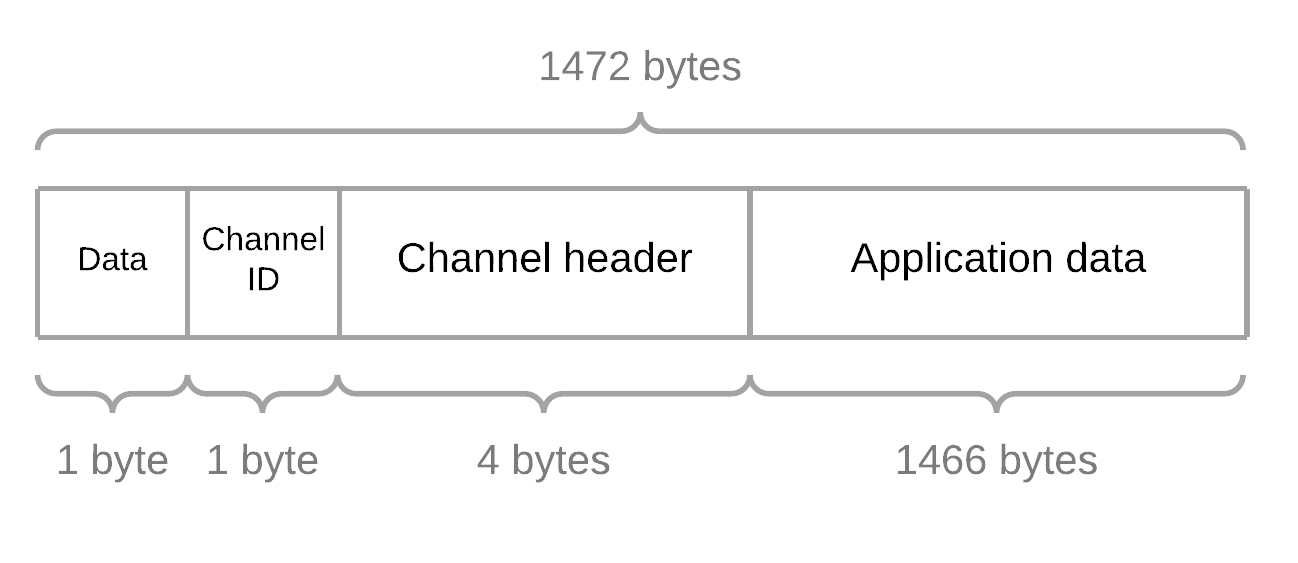
\includegraphics[scale=0.2]{Data-packet-structure}
	\caption{Data-packet structure}
	\label{fig:data-packet-structure}
\end{figure}


\subsubsection{Array pooling}
Fluid gameplay with no stuttering is essential for user experience. A minimum value of 60 frames per second\footnote{https://en.wikipedia.org/wiki/Frame\_rate} (FPS) is considered essential for a pleasant experience. Failing to render at least that many frames each second might result in noticeable lag, decreasing overall user satisfaction. This constraint means that all of the updates need to be performed in about 16 milliseconds. Consequently, this implies that expensive, long-running operations should be run as rarely as possible. One such operation is the process of garbage collection\footnote{https://en.wikipedia.org/wiki/Garbage\_collection\_(computer\_science)}, where all of the previously allocated memory that is no longer referenced gets freed.\\

However, garbage collection is only triggered when memory is no longer referenced. If we keep a reference to previously allocated memory and reuse it, no garbage collection will be performed. This type of memory reuse is called \textit{object pooling}\footnote{https://en.wikipedia.org/wiki/Object\_pool\_pattern} and is a standard practice in high-performance applications. As networked applications constantly keep sending packets back and forth (and packets are essentially just arrays of bytes), utilizing object pooling is perfectly suitable.\\

In our implementation, array pooling is implemented using an array of buckets. In this context, term \textit{bucket} means a collection of reusable arrays. Each bucket holds multiple arrays of same sizes and each subsequent bucket holds arrays of exponentially increasing capacities. First bucket holds arrays of size \textit{Packet.MaxSize}. Last bucket holds arrays of sizes \textit{Packet.MaxSize * 256}, which is maximum allowed size of a fragmented packet. This structure is shown at \ref{fig:array-pool-buckets}.


\begin{figure}[h!]
	\centering
	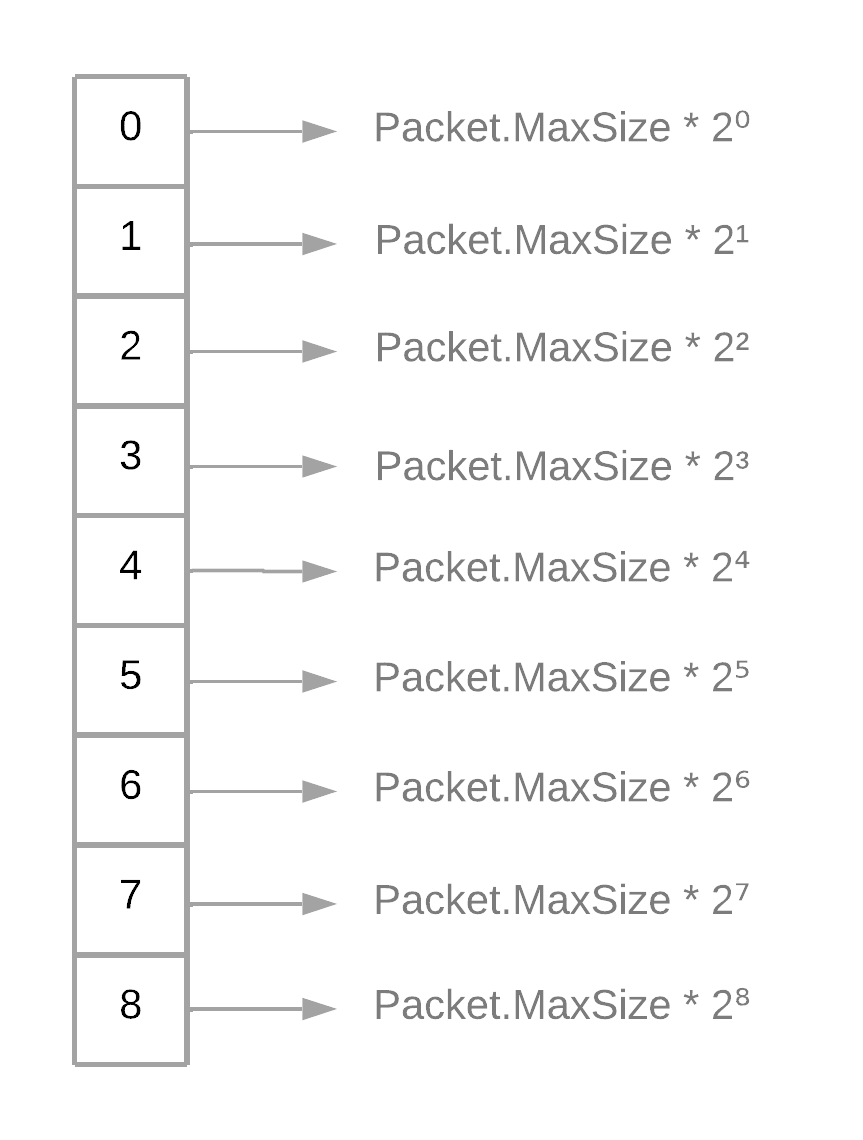
\includegraphics[scale=0.2]{Array-pool-buckets}
	\caption{Array pool buckets}
	\label{fig:array-pool-buckets}
\end{figure}



\subsection{Channels}
Channel represents a component that controls the way packets are sent and received. There are four fundamental problems that a channel can, but does not have to solve:

\begin{enumerate}
	\item \textbf{Order} - ability for the receiver to receive packets in order in which they were originally sent.
	\item \textbf{Duplication} - ability for receiver to detect and discard duplicate packets.
	\item \textbf{Reliability} - ability for sender to ensure that receiver received a packet.
	\item \textbf{Fragmentation} - ability for sender to divide a big packet into smaller packets called \textit{fragments} and for receiver to reassemble those into original big packet.
\end{enumerate}

\begin{center}
	\begin{table}[H]
		\centering
		
		\begin{tabular}{ |c|c|c|c|c|c| } 
			\hline
			Name & Order & Duplication & Reliability & Fragmentation \\ 
			\hline
			Unreliable        & - & - & - & - \\ 
			Sequenced         & Yes & Yes & - & - \\ 
			Reliable          & Yes & Yes & Yes & Yes \\ 
			\hline
		\end{tabular}
		
		\caption{Channel implementations and problems each implementation solves}
	\end{table}
\end{center}

Each channel also has a name associated with it and keeps track of bandwidth statistics, which is useful for diagnosing network usage. Information tracked by the channel are following state variables:

\begin{enumerate}
	\item \textbf{Packets sent} represents total number of packets sent through the channel.
	\item \textbf{Bytes sent} represents total number of bytes sent through the channel.
	\item \textbf{Packets received} represents total number of packets received on the channel.
	\item \textbf{Bytes received} represents total number of bytes received on the channel.
\end{enumerate}



\subsubsection{Unreliable channel}
Unreliable channel is the most basic channel type that does no processing of sent and received packets. Since it does not perform any logic, this channel type does not use any header bytes in the packet (\ref{fig:unreliable-packet-structure}). It acts as a pure UDP socket, therefore it does not provide any insurance:

\begin{enumerate}
	\item Packets can arrive out-of-order and receiver has no way of reassembling packets in order.
	\item Packets can be duplicated in the network and receiver has no way of knowing if it received a duplicate packet.
	\item Packets can be lost in the network and sender has no way of knowing if packet was potentially lost in transit.
	\item Packet size is limited as there is no support for fragmentation and reassembly.
\end{enumerate}

\begin{figure}[h!]
	\centering
	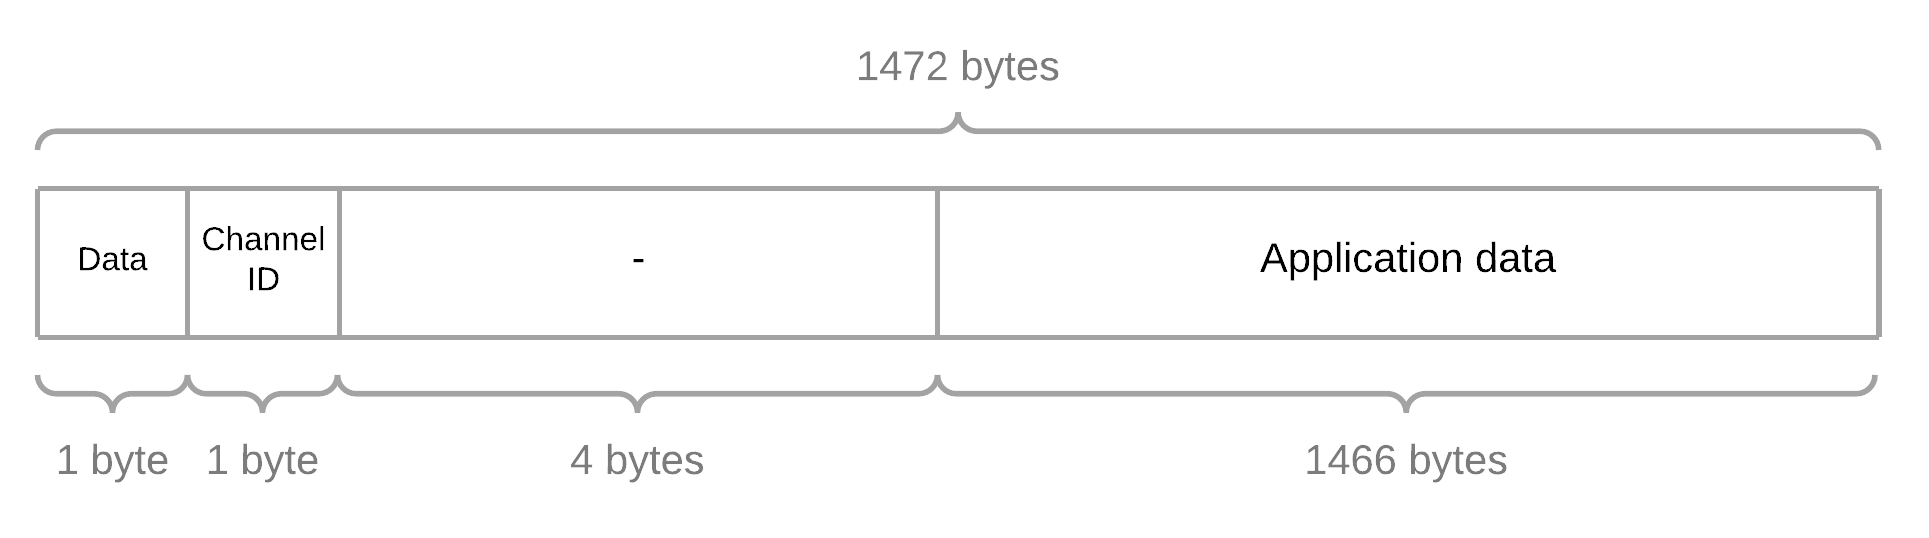
\includegraphics[scale=0.2]{Unreliable-packet-structure}
	\caption{Format of the packet sent through the unreliable channel.}
	\label{fig:unreliable-packet-structure}
\end{figure}



\subsubsection{Sequenced channel}
Sequenced channel solves two problems: order and duplication. It does so by attaching a unique number to each outgoing packet called \textit{local sequence number} (\ref{fig:sequenced-packet-structure}), which is a state variable maintained by the sending side of the channel. For each packet sent, local sequence number is incremented. 

\begin{figure}[h!]
	\centering
	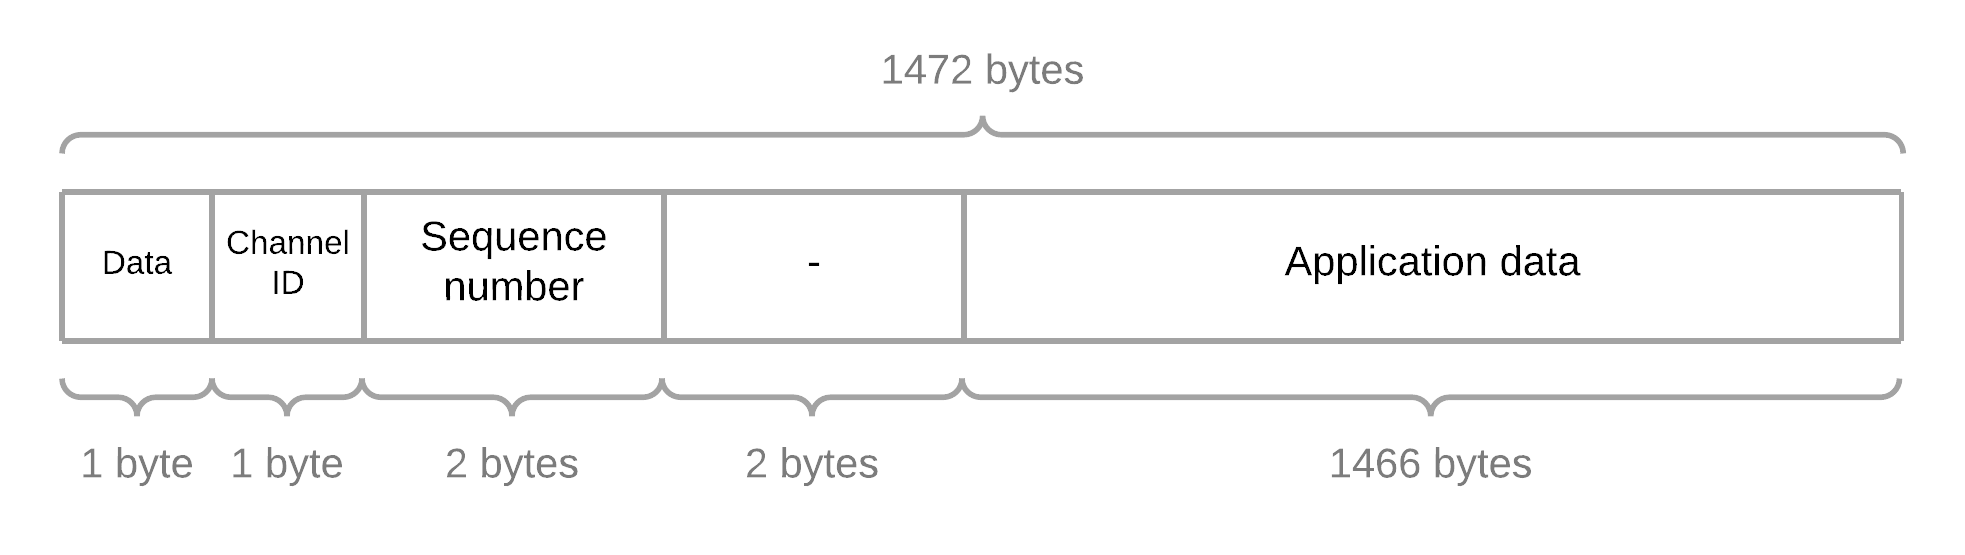
\includegraphics[scale=0.2]{Sequenced-packet-structure}
	\caption{Format of the packet sent through the sequenced channel.}
	\label{fig:sequenced-packet-structure}
\end{figure}

On the receiver side, another state variable is maintained: \textit{remote sequence number}. The remote sequence number holds the value of the highest received sequence number and this value is used to determine whether a newly received packet should be accepted or discarded. \\

Once a new packet is received, the sequence number is read from the packet. If the sequence number contained in the packet is greater than the remote sequence number, packet is accepted, otherwise it is discarded. \\

Another problem needs to be addressed: sequence number wrapping. As sequence numbers are stored in only 2 bytes, maximum sequence number value can be 65535. Once this sequence number is reached, next packet sequence number is going to wrap back to the minimum value of 0. Using naive approach of comparing raw sequence number values is going to produce wrong results; even though 65535 is numerically greater than 0, it logically is not. To solve this problem, the following algorithm is used to compare sequence numbers:

\begin{algorithm}[H]
	\caption{Comparing sequence numbers with wrapping}
	\textbf{Input:} First sequence number $seq1$, second sequence number $seq2$ \\
	\textbf{Output:} $true$ if $seq1$ is greater than $seq2$, $false$ otherwise \\
	
	\begin{algorithmic}
		\State $isGreaterRegular \gets seq1 > seq2 \AndWord seq1 - seq2 \leq 32767$
		\State $isGreaterWithWrap \gets seq1 < seq2 \AndWord seq2 - seq1 > 32767$ \\
		\Return $isGreaterRegular \OrWord isGreaterWithWrap$
	\end{algorithmic}
\end{algorithm}

Algorithm is based on a simple idea: if sequence number values are close numerically, wrapping did not occur. Sequence numbers are close if absolute value of their difference is smaller or equal to half of the full sequence number range.


\subsubsection{Reliable channel}
Reliable channel solves all four problems: order, duplication, reliability and fragmentation. The rest of this section is going to cover in detail how reliability and fragmentation were solved.\\

To solve reliability, packet acknowledgments and re-transmission concepts are borrowed from TCP. The idea is that each packet sent needs to be acknowledged by the receiver. If packet is not acknowledged in a certain amount of time, it is considered lost and will be re-transmitted (\ref{fig:resend-diagram}). A packet that has been sent, but not yet acknowledged by the receiver is called a \textit{pending packet}. \\

Each pending packet internally maintains a timer that will, if expired, automatically resend the packet. If acknowledgment is received before timer expires, timer is canceled and pending packet is removed from the collection of active pending packets. To prevent sending packets \textit{ad infinitum}, each pending packet internally counts number of re-transmission attempts. If the counter exceeds maximum number of attempts (value which is defined by the channel), connection is deemed as lost. \\

\begin{figure}[H]
	\centering
	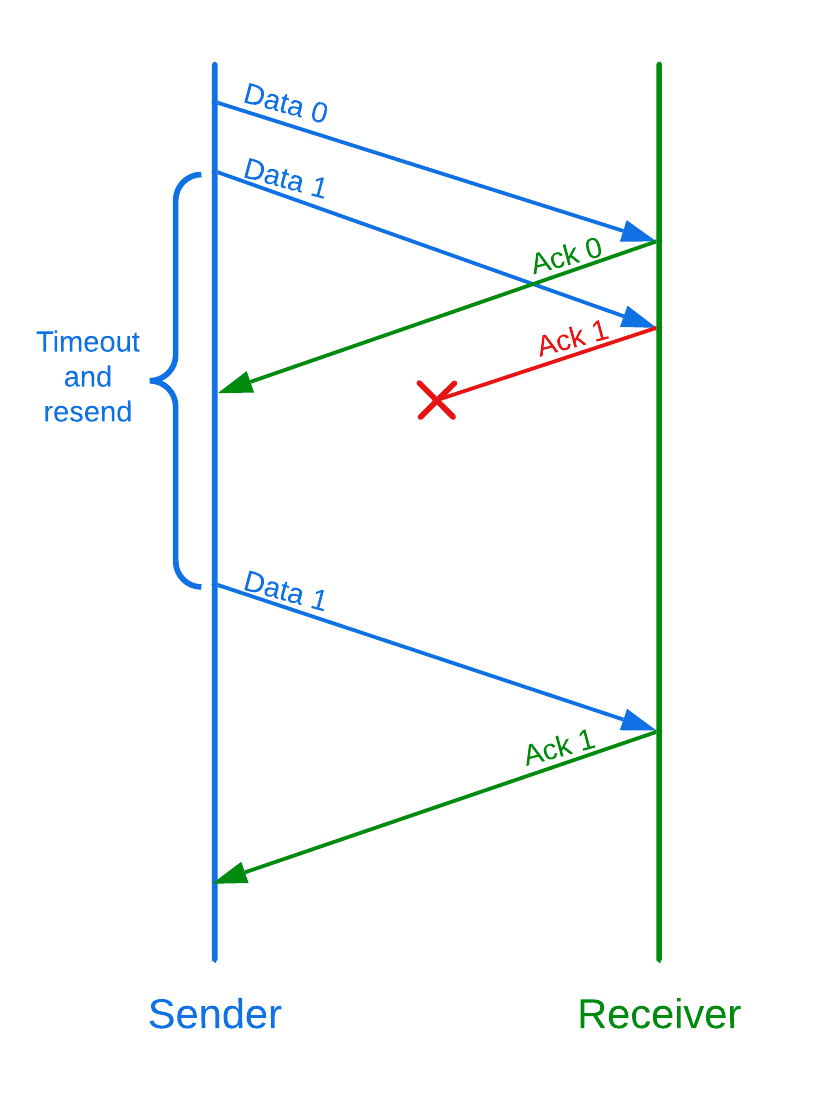
\includegraphics[scale=0.3]{Resend-diagram}
	\caption{Resend diagram that shows how data and acknowledgment packets are sent and received. Diagram shows that data-packet 0 was successfully acknowledged and did not require a resend. Meanwhile, acknowledgment of data-packet 1 was lost in transit, which in turn made sender's timer time-out, causing data-packet 1 to be resent.}
	\label{fig:resend-diagram}
\end{figure}

On the receiving side of the channel, array of received packets is maintained. It is an array that is updated in the following manner: for each received packet, sequence number is read from the header. If array slot at index which is equal to sequence number is empty, that means received packet is not a duplicate and is stored in the array. If the slot is already filled, that means received packet is a duplicate and is discarded. \\

For each received packet, duplicate or not, acknowledgment is sent to the sender. Acknowledgment packet has the ability to acknowledge multiple packets at once. Naive approach would be to simply send an array of several most recently received packet sequence numbers. Since each sequence number is a 16-bit integer, that approach is very bandwidth inefficient. Much more efficient approach is to use so called \textit{anchor sequence number} combined with additional acknowledgment bit-field (\ref{fig:ack-packet-structure}). \\

Anchor sequence number is an actual 16-bit sequence number and it is equal to the sequence number of the most recently received packet. Acknowledgment bit-field is a bit-field in which each bit is responsible for acknowledging a sequence number relative to anchor. Concretely, first bit is responsible for indicating whether packet with sequence number \textit{anchor - 1} has been received. If bit is set, it means packet was received, otherwise it wasn't. In general, bit at position \textit{n} is responsible for indicating whether packet with sequence number \textit{anchor sequence number - n} has been received. With this approach, 8 previous sequence numbers can be acknowledged using only 1 additional byte of data. This approach achieves perfect entropy\footnote{https://en.wikipedia.org/wiki/Entropy\_(information\_theory)}.\\

\begin{figure}[H]
	\centering
	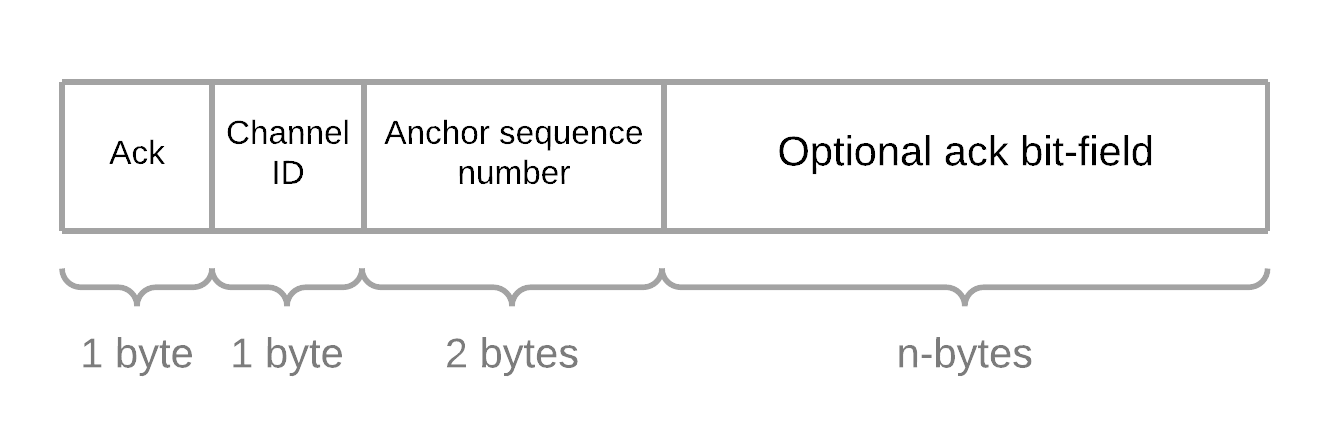
\includegraphics[scale=0.25]{Ack-packet-structure}
	\caption{Format of the acknowledgment packet sent through the reliable channel.}
	\label{fig:ack-packet-structure}
\end{figure}

In order for receiver to receive packets in actual order they were originally sent, another state variable is used: \textit{receive sequence number}. It represents the next expected packet sequence number. Once a packet with that sequence number is received, packet is forwarded to the library user and receive sequence number is incremented. If packet is received out-of-order (for example, packet with number 7 is received before 6), packet is buffered for later (\ref{fig:ordered-receive}).

\begin{figure}[H]
	\centering
	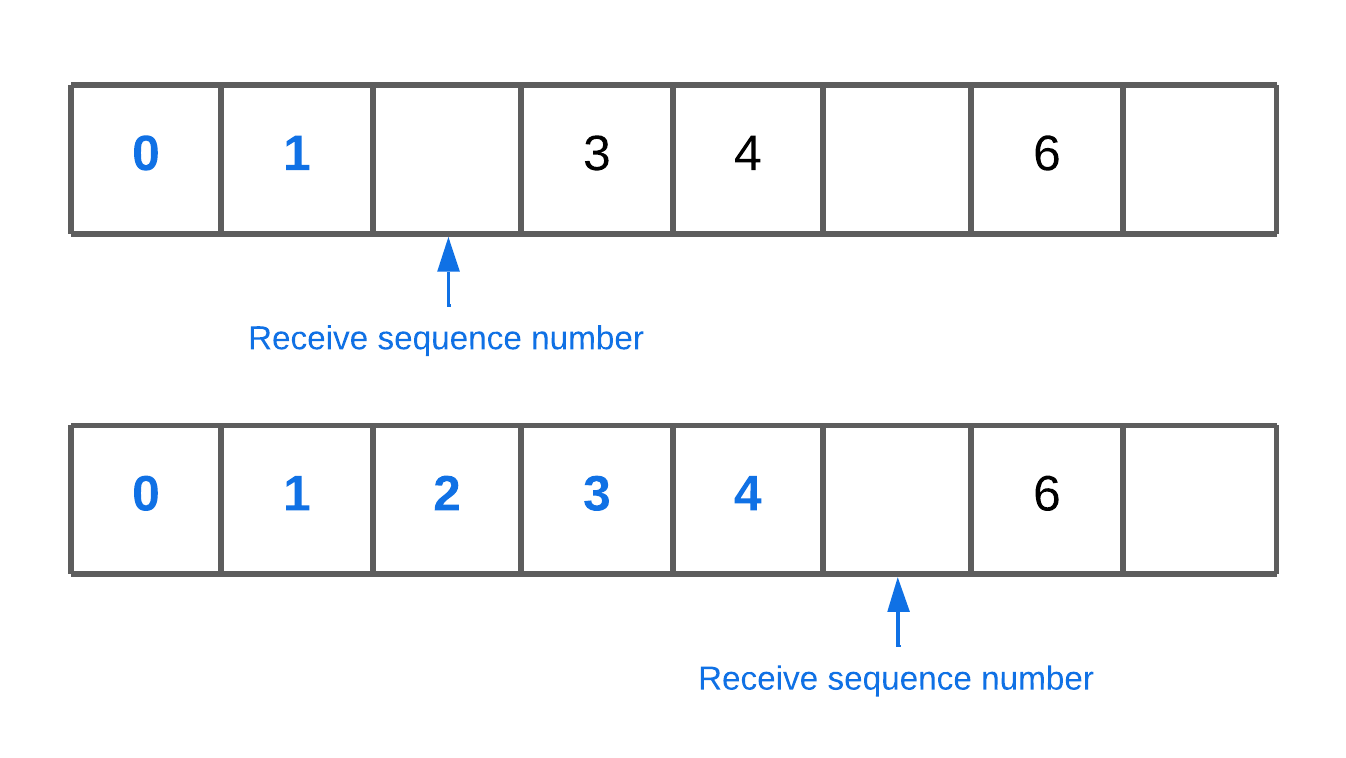
\includegraphics[scale=0.25]{Ordered-receive}
	\caption{Ordered receive implemented using \textit{receive sequence number}. Array slots that have numbers in it represent already received and stored packets, while empty slots are packets that haven't been received yet. Blue numbers represent packets that have been forwarded to library user. First array shows that sequence number 2 is expected and that packets 3, 4 and 6 have been already received, but haven't been forwarded to the user (as forwarding would violate order since packet 2 still hasn't been received). Second array shows what happens when packet 2 is received. Packet 2 is forwarded, but also 3 and 4 since those packets have been received earlier. At the end of it, next expected sequence number is 5.}
	\label{fig:ordered-receive}
\end{figure}

With the previously described system packets are always received in-order and are guaranteed to be delivered (or connection times-out if maximum number of resend attempts are exceeded). This channel property allows implementation of another very useful feature: fragmentation and reassembly of big packets \cite{GafferOnGames:Sending-large-blocks-of-data}.\\

Fragmentation is a process of breaking up a big packet into multiple smaller packets called \textit{fragments} which can be easily transferred over the network. A big packet is defined as a packet whose size exceeds maximum packet size \eqref{eq:max_packet_size}. Fragmentation is performed by the sending side of the channel. Reassembly is the reverse process: combining fragments into the original big packet. Reassembly is performed by the receiving side of the channel (\ref{fig:fragmentation-and-reassembly}). \\

\begin{figure}[H]
	\centering
	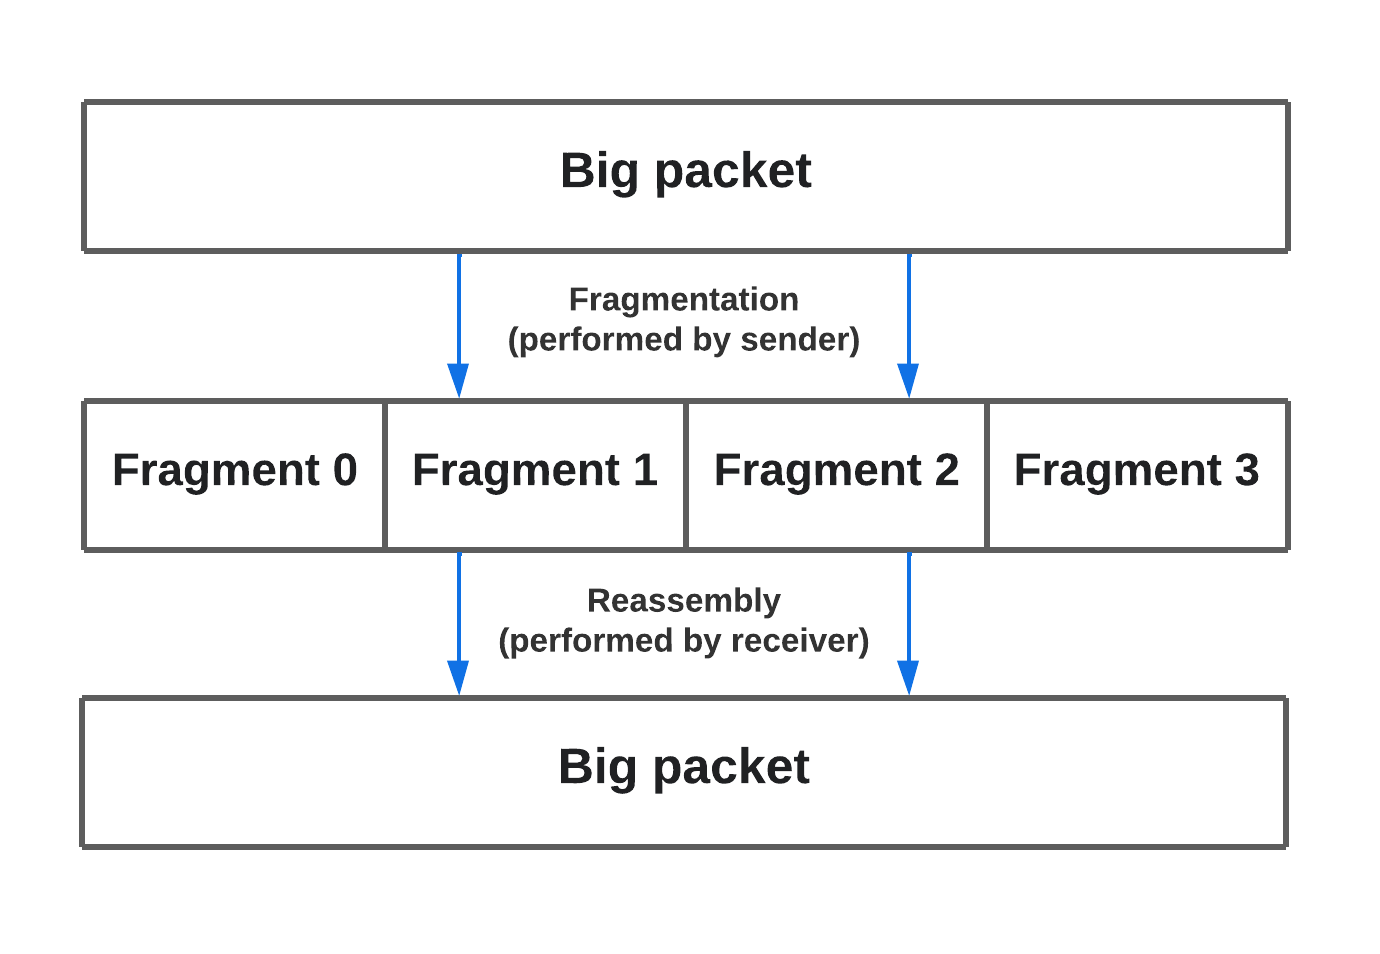
\includegraphics[scale=0.3]{Fragmentation-and-reassembly}
	\caption{Simple flow diagram of fragmentation and reassembly.}
	\label{fig:fragmentation-and-reassembly}
\end{figure}

In order to support fragmentation and reassembly, additional fields need to be attached to each packet. First field is \textit{fragment index} which defines a position in the original big packet. Second field is \textit{fragment count} that states how many fragments a big packet consists of (\ref{fig:reliable-packet-structure}).

\begin{figure}[H]
	\centering
	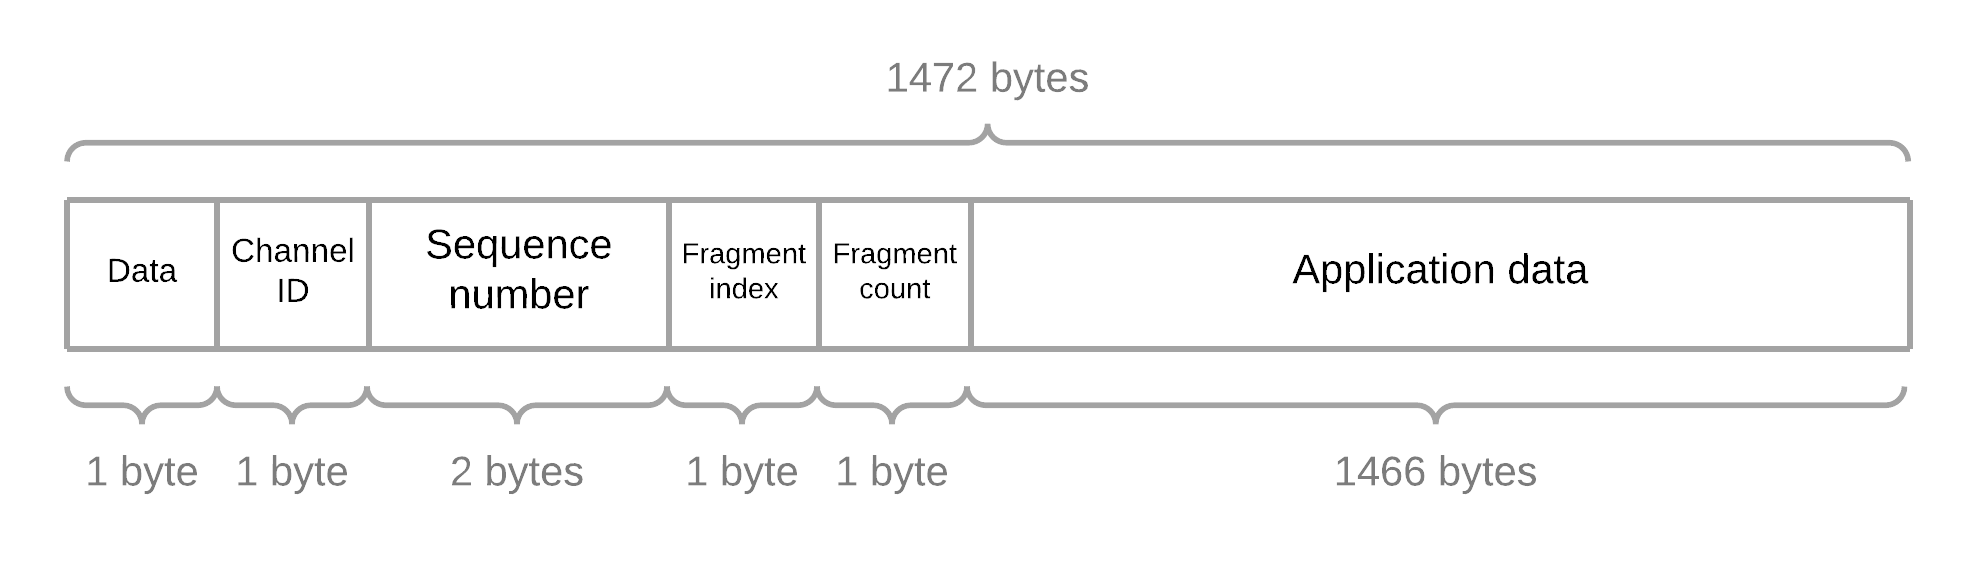
\includegraphics[scale=0.2]{Reliable-packet-structure}
	\caption{Format of the packet sent through the reliable channel.}
	\label{fig:reliable-packet-structure}
\end{figure}

Fragmentation on the sender side of the channel is performed as follows: each time a packet is being sent, total number of fragments required is calculated (based on the packet size). If packet consists of only a single fragment, that means fragmentation is not needed and packet is sent as is (with fragment index set to 0 and fragment count set to 1). If packet consists of multiple fragments, big packet's payload is distributed into multiple fragments (each storing only a fraction of the big packet) and then each fragment is sent. \\

Reassembly on the receiver side of the channel is performed as follows: if a fragment with count of 1 is received, it is immediately forwarded to the user. If fragment count is greater than 1, receiver attempts to reassemble original big packet. It can only do so if all of the fragments have been received (\ref{fig:fragmentation-received-packets}).

\begin{figure}[H]
	\centering
	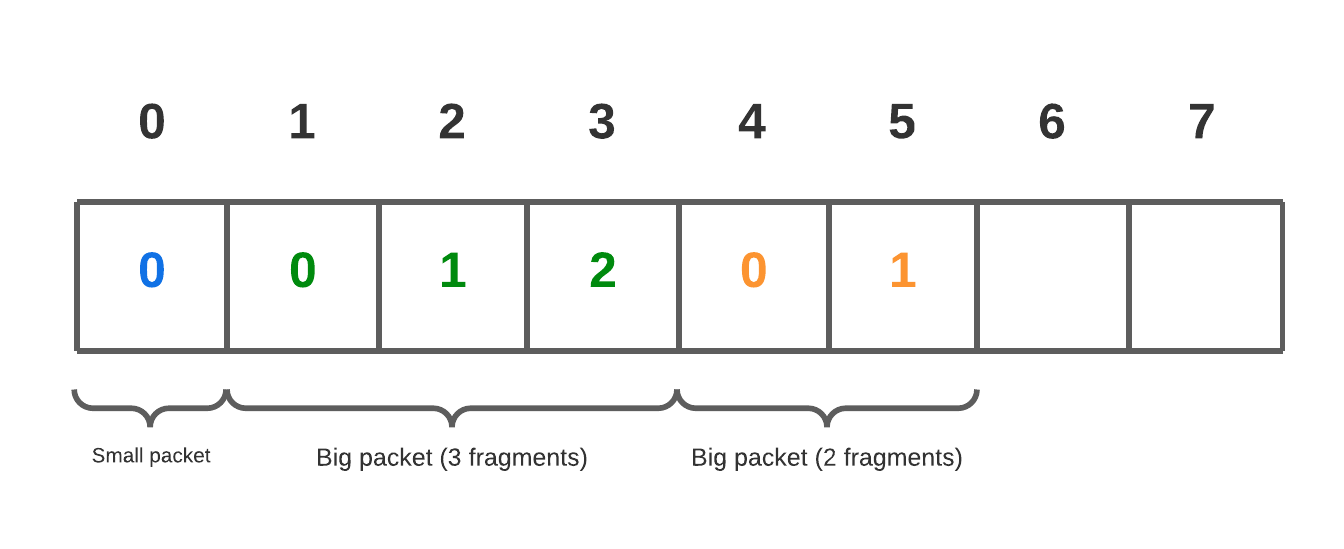
\includegraphics[scale=0.3]{Fragmentation-pending-packets}
	\caption{Example of received packets array combined with fragmentation and reassembly system. Numbers above the array represent packet sequence numbers. Numbers in the array slots represent fragment indexes. Numbers with the same color belong to the same original big packet. Once receiver receives all of the required fragments (which it can deduce based on the fragment count attached to each fragment), it can reassemble original big packet.}
	\label{fig:fragmentation-received-packets}
\end{figure}

This fragmentation and reassembly implementation allows users to efficiently and safely send packets with sizes up to $1466 \times 255 = 373830 \; bytes$.



\subsection{Connection}
Connection represents a link between two network nodes \cite{GafferOnGames:ClientServerConnection}. It is a higher level component that has multiple responsibilities:

\begin{enumerate}
	\item Holds an array of channels and is responsible for forwarding packets to the corresponding channel.
	\item Calculates round-trip time by sending ping packets and automatically performs time-out if no valid response is received in certain amount of time.
	\item Keeps track of bandwidth statistics (total number of packets/bytes that were sent/received).
\end{enumerate}

Each connection can have up-to 256 channels. Channels are differentiated by their ID, which is a single byte value (\ref{fig:connection-channels}).

\begin{figure}[H]
	\centering
	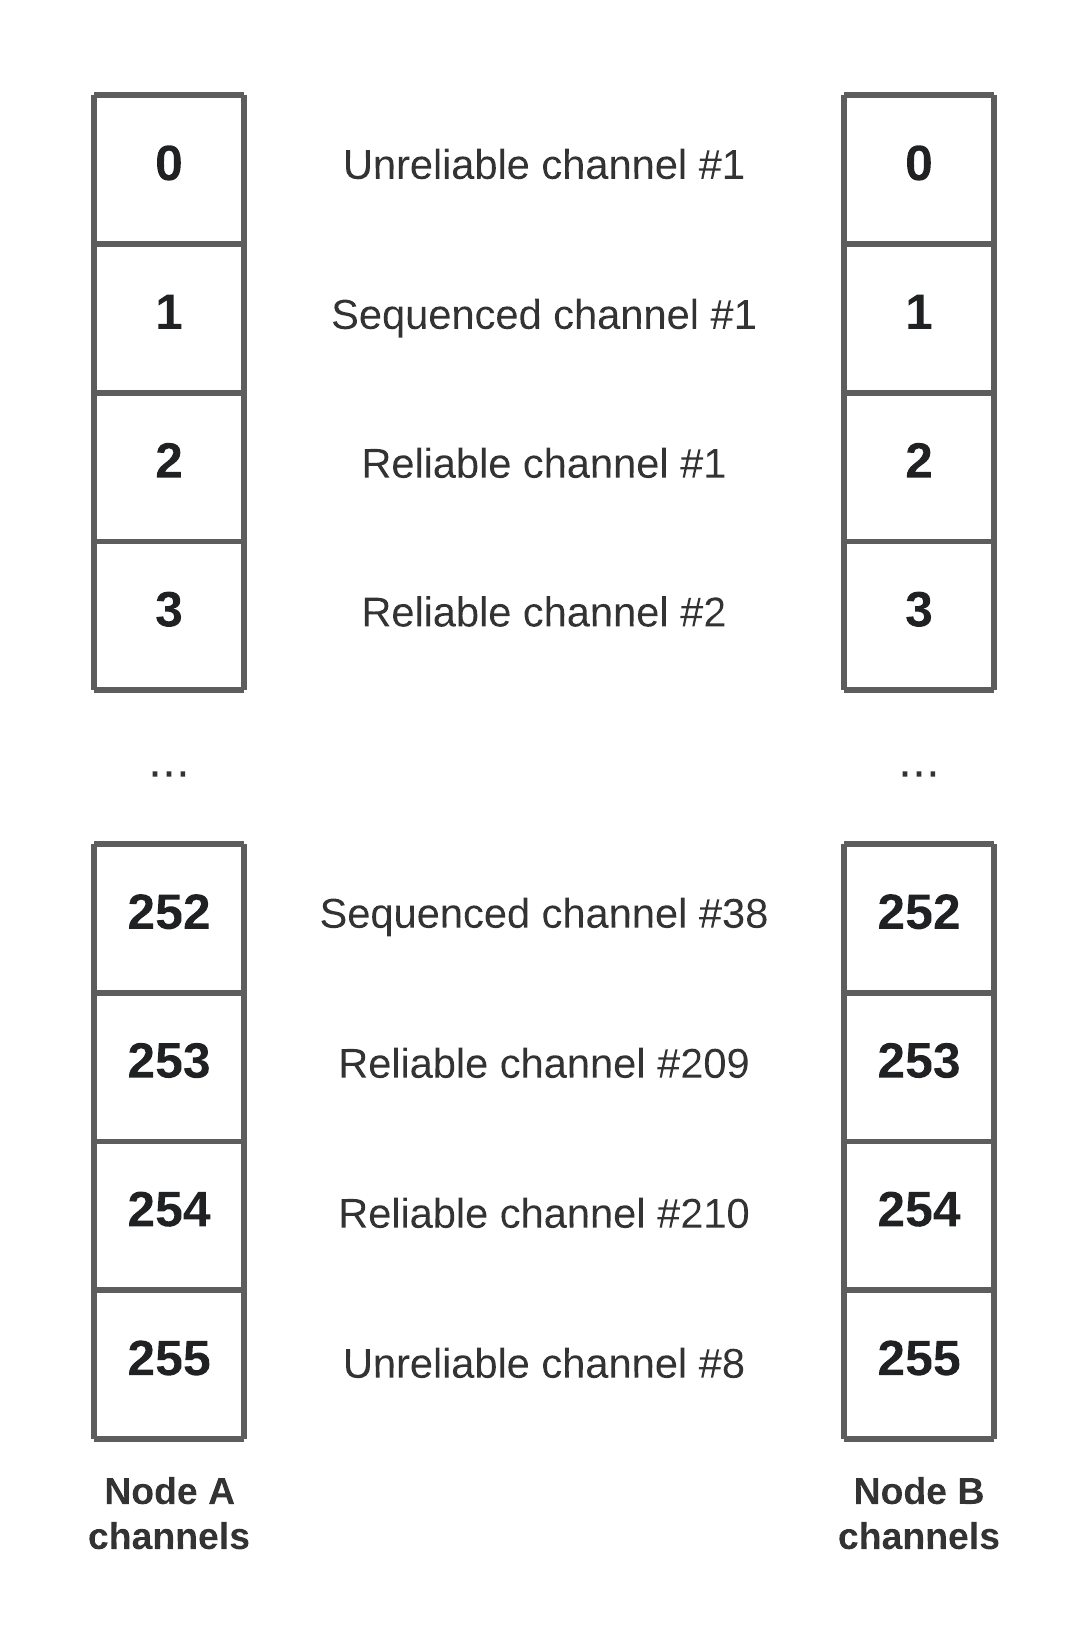
\includegraphics[scale=0.25]{Connection-channels}
	\caption{Example of channel array that is maintained by the connection.}
	\label{fig:connection-channels}
\end{figure}

Round-trip time is calculated by periodically sending packets with \textit{Ping} header type and attaching an incrementing identifier to the packet. Time of the sent ping is also stored in order to calculate round-trip time once response is received. Upon receiving a ping packet, receiver responds by sending a packet with \textit{Pong} header type and including identifier of the received ping packet. Once original sender receives the pong packet, it calculates round-trip time by taking the time difference between ping send and pong receive timestamps.



\subsection{Nodes}
To tie it all together, an actual network node is required. A network node represents a fundamental building block of any network graph that can send and receive data. A graph\footnote{https://en.wikipedia.org/wiki/Graph\_theory\#Graph} consists of vertices (which are represented by nodes) and edges (which are represented by connections) (\ref{fig:network-graph}).

\begin{figure}[H]
	\centering
	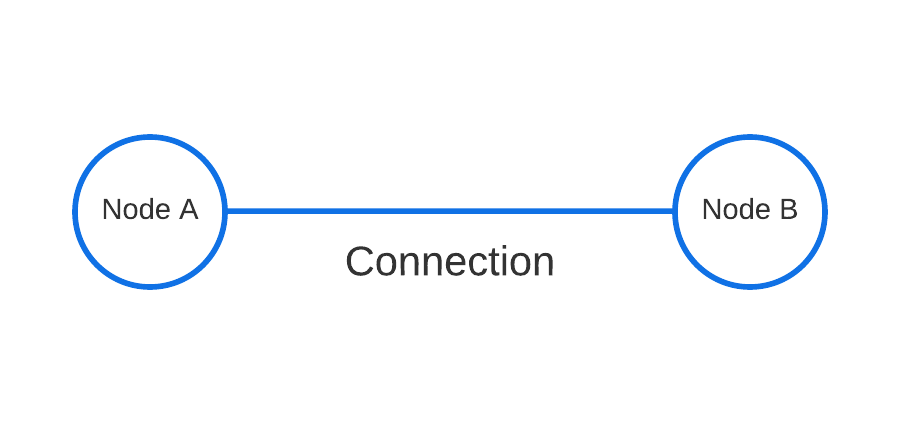
\includegraphics[scale=0.35]{Connection}
	\caption{Visual representation of a simple network graph.}
	\label{fig:network-graph}
\end{figure}

\subsubsection{Client}
Client represents a network node that has one to one relationship with the server. Client node never directly communicates with any other client nodes, only with the server. Client exposes a simple API\footnote{https://en.wikipedia.org/wiki/API} for connecting to the server, sending packets and disconnecting from the server.

\begin{table}[H]
	\centering
	\begin{tabular}{|c|c|}
		\hline
		\textbf{Method} & \textbf{Description}                                                                                            \\ \hline
		Connect         & \begin{tabular}[c]{@{}c@{}}Attempts to establish a\\ connection with the server.\end{tabular}                   \\ \hline
		Send            & Sends a packet to the server.                                                                                   \\ \hline
		Disconnect      & \begin{tabular}[c]{@{}c@{}}Disconnects from the server and\\ stops listening for incoming packets.\end{tabular} \\ \hline
	\end{tabular}
	\caption{Client API.}
	\label{table:client-api}
\end{table}

Client also raises important events that occurred during runtime\footnote{https://en.wikipedia.org/wiki/Runtime\_(program\_lifecycle\_phase)}, which are listed in table \ref{table:client-events}.

\begin{table}[H]
	\centering
	\begin{tabular}{|c|c|}
		\hline
		\textbf{Event} & \textbf{Description}                                                                                                              \\ \hline
		Connecting     & \begin{tabular}[c]{@{}c@{}}Invoked each time client starts the process of\\ establishing connection with the server.\end{tabular} \\ \hline
		Connected      & \begin{tabular}[c]{@{}c@{}}Invoked each time client\\ successfully connects to the server.\end{tabular}                           \\ \hline
		ConnectFailed  & \begin{tabular}[c]{@{}c@{}}Invoked each time client fails to\\ establish a connection with the server.\end{tabular}               \\ \hline
		PacketReceived & \begin{tabular}[c]{@{}c@{}}Invoked each time a data-packet\\ is received from the server.\end{tabular}                            \\ \hline
		Disconnected   & \begin{tabular}[c]{@{}c@{}}Invoked each time client\\ disconnects from the server.\end{tabular}                                   \\ \hline
	\end{tabular}
	\caption{All of the possible events that can be raised by a client node.}
	\label{table:client-events}
\end{table}

\subsubsection{Server}
Server represents a network node that has one to many relationship with clients. Server node never communicates with any other server nodes. Server exposes a simple API for starting the server, sending packets to one or more clients, kicking specific clients and stopping the server.

\begin{table}[H]
	\centering
	\begin{tabular}{|c|c|}
		\hline
		\textbf{Method} & \textbf{Description}                                                                                         \\ \hline
		Start           & Starts listening for incoming client packets.                                                                \\ \hline
		SendToOne       & Sends a packet to one specific client.                                                                       \\ \hline
		SendToMany      & Sends a packet to many clients.                                                                              \\ \hline
		SendToAll       & Sends a packet to all connected clients.                                                                     \\ \hline
		Kick            & Deliberately disconnects specific client.                                                                    \\ \hline
		Stop            & \begin{tabular}[c]{@{}c@{}}Disconnects all clients and ignores\\ any further incoming packets.\end{tabular} \\ \hline
	\end{tabular}
	\caption{Server API.}
	\label{table:server-api}
\end{table}

Server also raises important events that occurred during runtime, to which many subscribers can listen to.

\begin{table}[H]
	\centering
	\begin{tabular}{|c|c|}
		\hline
		\textbf{Event}     & \textbf{Description}                                                                                                   \\ \hline
		Started            & \begin{tabular}[c]{@{}c@{}}Invoked each time server starts and\\ begins listening for client connections.\end{tabular} \\ \hline
		ClientConnected    & \begin{tabular}[c]{@{}c@{}}Invoked each time a new client\\ connects to the server.\end{tabular}                       \\ \hline
		ClientDisconnected & \begin{tabular}[c]{@{}c@{}}Invoked each time an already connected\\ client disconnects from the server.\end{tabular}   \\ \hline
		PacketReceived     & \begin{tabular}[c]{@{}c@{}}Invoked each time a data-packet\\ is received from a client.\end{tabular}                   \\ \hline
		Stopped            & \begin{tabular}[c]{@{}c@{}}Invoked each time server stops and no\\ longer listens for client connections.\end{tabular} \\ \hline
	\end{tabular}
	\caption{All of the possible events that can be raised by a server node.}
	\label{table:server-events}
\end{table}

\subsubsection{Simulation}
When building a networking application using local network, connection is almost always going to be flawless. There will be no packet loss, latency will be minuscule and there will generally be no problems.\\

However, real-life networks are unpredictable; packet-loss will occur and latency is going to vary. In order to test how your application would behave under those real network conditions, optional network simulation can be enabled. It allows each node to specify artificial packet-loss and any amount of latency.


\chapter{High-level library}
This chapter explains in detail components that together make-up high-level library developed for the Unity\footnote{https://unity.com/} game-engine.

\section{Network Manager}
\textit{NetworkManager} is a central component of the high-level library that has several responsibilities:

\begin{enumerate}
	\item It contains network configuration.
	\item It contains and manages all of the networked objects in the scene.
	\item It handles all of the internal library packets.
\end{enumerate}

\subsection{Network configuration}
In order to help user easily configure networking settings, it is all in one place - in the NetworkManager component (\ref{fig:network-manager-inspector}). It is also the only component that implements the singleton pattern\footnote{https://en.wikipedia.org/wiki/Singleton\_pattern}, allowing convenient access from anywhere in the application.\\

\textit{Run In Background} set to \textit{true} ensures that application is going to run even if it does not have focus\footnote{https://en.wikipedia.org/wiki/Focus\_(computing)}. \textit{Don't Destroy On Load}\footnote{https://docs.unity3d.com/ScriptReference/Object.DontDestroyOnLoad.html} set to \textit{true} marks NetworkManager as scene-persistent - changing scenes will not destroy the instance. \textit{Network Prefabs Path} defines where all of the object templates that can be spawned over the network are located.\\

Next-up there are client settings - IP address and port to which connect attempt should be made. Server settings define listen port and maximum number of client connections. Both client and server can then also set-up virtual network simulation - packet-loss, minimum and maximum latency.\\

\textit{RPC Naming Convention} allows the user to specify how RPC methods should be named in pursue of cleaner code. \textit{Debug Information} helps user to detect potential packet or network object leaks during runtime and provides useful information such as registered client and server packet handlers and types used by the serialization system.

\begin{figure}[H]
	\centering
	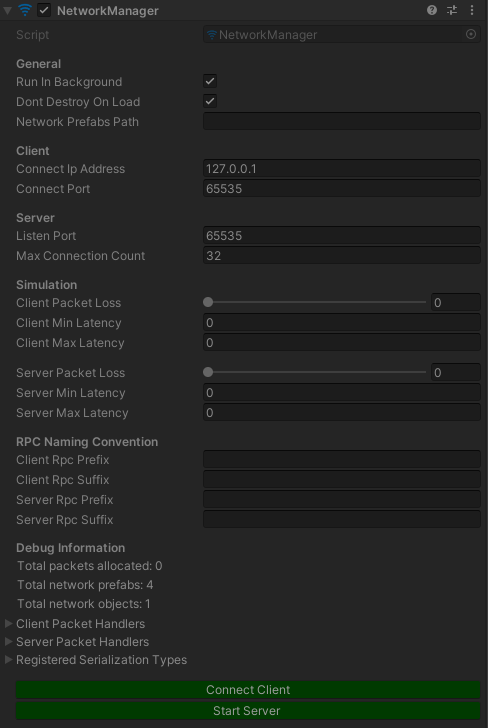
\includegraphics[scale=0.85]{NetworkManager-inspector}
	\caption{NetworkManager shown in the Unity inspector.}
	\label{fig:network-manager-inspector}
\end{figure}

\subsection{Network objects}
NetworkManager stores and keeps track of all active networked objects in the current scene. It separates them into two groups: scene objects and spawned objects. Scene objects are networked objects that are baked into the scene and both client and server have them at the start of the game. Runtime objects are networked objects that are spawned during runtime by the manager on the server side. In order to uniquely identify objects over the network, manager also assigns each object a unique number called \textit{object ID}. \\

\subsubsection{Spawning}
In order for manager to be able to spawn objects over the network, each process instance has to contain information about which objects can be spawned. This information is stored in a dictionary which maps unique IDs to corresponding prefabs that can be spawned (\ref{fig:network-manager-prefabs}).

\begin{figure}[H]
	\centering
	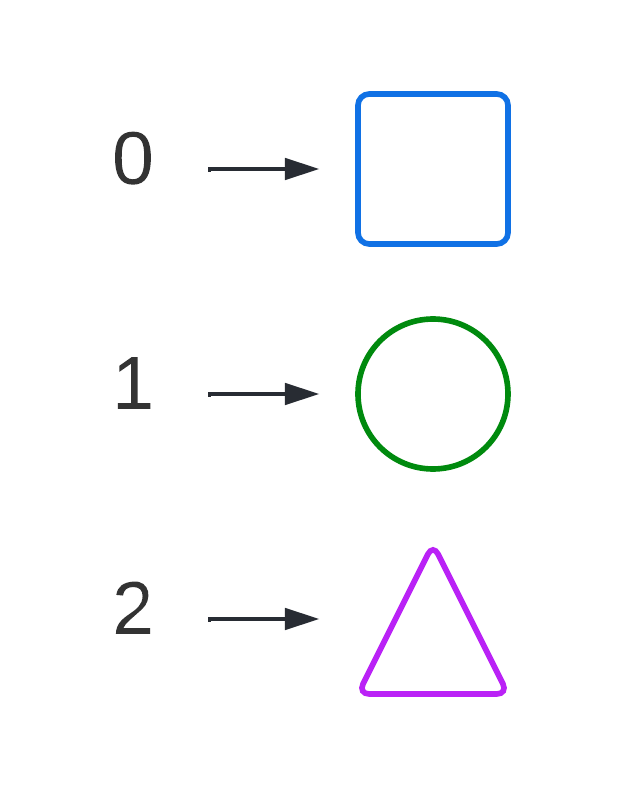
\includegraphics[scale=0.3]{NetworkManager-prefabs}
	\caption{Example of prefabs that are registered in the NetworkManager - each prefab has been assigned an ID by the manager. For example, if manager wants to spawn a green circle over the network, all it has to do is send prefab ID and object ID to the clients which will be able to recreate their own green circles using local ID-prefab dictionary.}
	\label{fig:network-manager-prefabs}
\end{figure}

With such structure, spawning is a simple process: manager creates an object from the prefab template, assigns it a unique object ID, stores it in a local dictionary and broadcasts prefab ID and object ID to all of the clients so their local managers can do the same. This process is encapsulates inside a single network manager method call.

\subsubsection{Destroying and toggling}
Destroying an object over the network is an even simpler process than spawning - manager destroys local networked object by ID and simply broadcasts the destroyed object ID so all the clients can destroy their own local copy of the object. \\

Toggling is the process of enabling or disabling an object. Similarly to destroying, all that has to be done to toggle an object over the network is to perform it locally and broadcast to other clients object ID and flag that indicates whether object is enabled or disabled.

\subsubsection{Library packets}
To perform all of the actions described by the previous sections and more, manager has to handle many packet types. Each packet type is responsible for one type of action and carries its own unique payload.

\begin{table}[H]
	\centering
	\resizebox{\textwidth}{!}{
		\begin{tabular}{|c|c|c|}
			\hline
			\textbf{Packet}     & \textbf{Description}                                                                                                                                      & \textbf{Payload}                                                                             \\ \hline
			Object Scene Create & \begin{tabular}[c]{@{}c@{}}Sent by the server to the client when a client joins and\\ needs to recreate an already existing networked scene.\end{tabular} & List of networked objects                                                                    \\ \hline
			Object Spawn        & \begin{tabular}[c]{@{}c@{}}Sent by the server to the client when\\ an object should be spawned.\end{tabular}                                              & \begin{tabular}[c]{@{}c@{}}Prefab ID, Object ID,\\ Transform\end{tabular}                    \\ \hline
			Object Owner        & \begin{tabular}[c]{@{}c@{}}Sent by the server to the client to give\\ or take ownership of the specific network object.\end{tabular}                      & Object ID, Is owner                                                                          \\ \hline
			Object Update       & \begin{tabular}[c]{@{}c@{}}Sent by the server to the client each update\\ tick when there are any object variable updates.\end{tabular}                   & Object ID, Variables                                                                         \\ \hline
			Object Transform    & \begin{tabular}[c]{@{}c@{}}Sent by the server to the\\ client to update object's transform.\end{tabular}                                                  & \begin{tabular}[c]{@{}c@{}}Object ID, Behavior index,\\ Transform\end{tabular}               \\ \hline
			Object Toggle       & \begin{tabular}[c]{@{}c@{}}Sent by the server to the client when a\\ networked object should be enabled or disabled.\end{tabular}                         & Object ID, Is enabled                                                                        \\ \hline
			Object Destroy      & \begin{tabular}[c]{@{}c@{}}Sent by the server to the client when\\ a networked object should be destroyed.\end{tabular}                                   & Object ID                                                                                    \\ \hline
			Rpc                 & \begin{tabular}[c]{@{}c@{}}Sent by the client to the server or server to \\ the client when invoking a remote procedure call.\end{tabular}                & \begin{tabular}[c]{@{}c@{}}Object ID, Behavior index,\\ Rpc hash and parameters\end{tabular} \\ \hline
		\end{tabular}
	}
	\caption{Internal packet types handled by the NetworkManager component.}
	\label{table:network-manager-packets}
\end{table}



\section{Network Object}
\textit{NetworkObject} (\ref{fig:network-object-example}) is a one of the core components of the high-level library. As such, it has multiple crucial purposes:

\begin{enumerate}
	\item It explicitly marks object as an entity that requires networking functionality, separating it from regular, non-networked entities.
	\item It contains a unique identifier of the object in a networked environment, making that object referable by multiple processes.
	\item It contains prefab\footnote{https://docs.unity3d.com/Manual/Prefabs.html} information from which object can be replicated over multiple processes.
	\item It contains ownership information, allowing user of the library to develop components which can only be executed by the object owner.
	\item It maintains a list of behavior components which provide concrete networked functionality.
\end{enumerate}

Even though it is one of the core components, on its own, it does not do much. It acts as a simple container of \textit{prefab ID} (identifier of the template from which the networked object has been created), \textit{object ID} (unique identifier of the specific network object instance) and \textit{ownership flag} (if set to true, object can be controlled by the local process, otherwise it can't).

\begin{figure}[H]
	\centering
	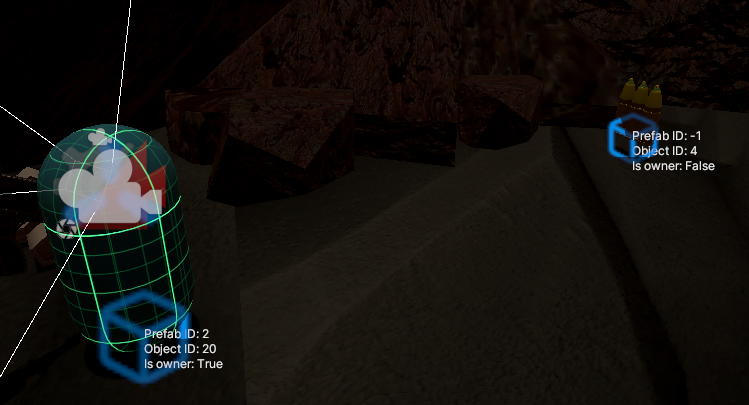
\includegraphics[scale=0.6]{NetworkObject-example}
	\caption{NetworkObject gizmos drawn in the Unity scene-view, allowing developer to easily view all of the networked objects and their information.}
	\label{fig:network-object-example}
\end{figure}

\section{Network Behavior}
\textit{NetworkBehavior} is an abstract component that allows and makes it easy for library user to implement arbitrary networked functionality. It is a class that extends \textit{MonoBehaviour}\footnote{https://docs.unity3d.com/ScriptReference/MonoBehaviour.html} and exposes two powerful features: state synchronization and remote procedure calls.

\subsection{State synchronization}
State synchronization is automatic distribution of modified state to each process in a networked environment. It abstracts away the need to create custom packets for each state variable present in the networked simulation. This section explains how such feature is achieved. \\

At the core of state synchronization feature is a concept incremental updates\footnote{https://en.wikipedia.org/wiki/Incremental\_computing} - only variables that have changed need to be synced. Since primitive types such as integers do not have a way to listen for their changes, a new generic wrapper type is introduced - \textit{NetworkVariable<T>} (where T represents variable's data-type). This system is a combination of Unity's previous \cite{Unity:UNet-SyncVar} and current \cite{Unity:NetworkVariable} state synchronization solutions.\\

\begin{figure}[H]
	\centering
	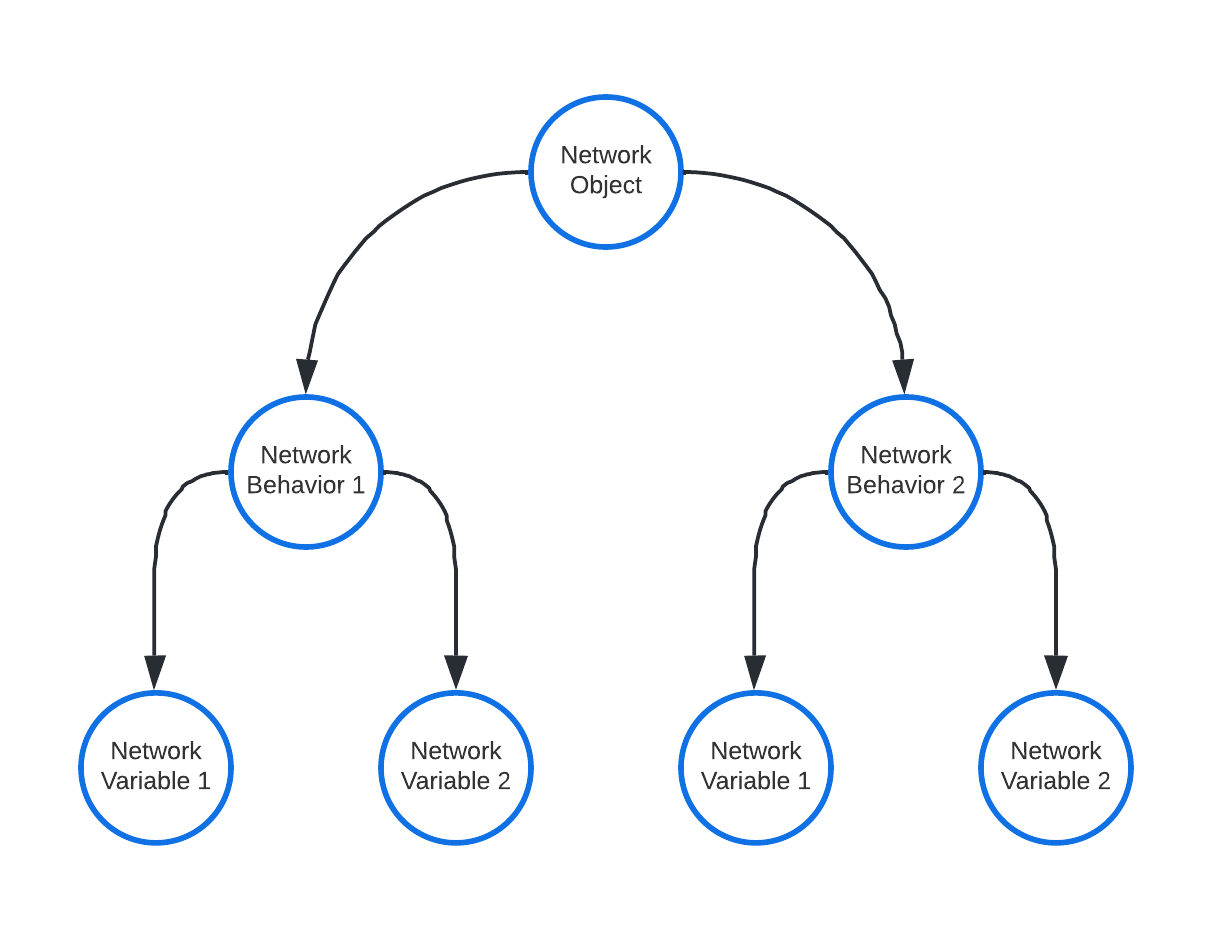
\includegraphics[scale=0.22]{NetworkObject-tree}
	\caption{NetworkObject hierarchy example - each networked object contains one or more behaviors and each behavior contains zero or more networked variables.}
	\label{fig:network-object-tree}
\end{figure}

NetworkVariable is a simple component that encapsulates a single state variable, keeps track of whether that variable has been modified and has the ability to serialize and deserialize the wrapped value. If state variable has been modified, it is going to fire an event. This event is important as it is going to notify NetworkBehavior that contains the variable of the change. In turn, behavior is going to notify NetworkObject of the change (which is possible because of a structured hierarchy \ref{fig:network-object-tree}) and that object is going to be added to a collection of objects that need to be synced (\ref{fig:network-object-propagation}).

\begin{figure}[H]
	\centering
	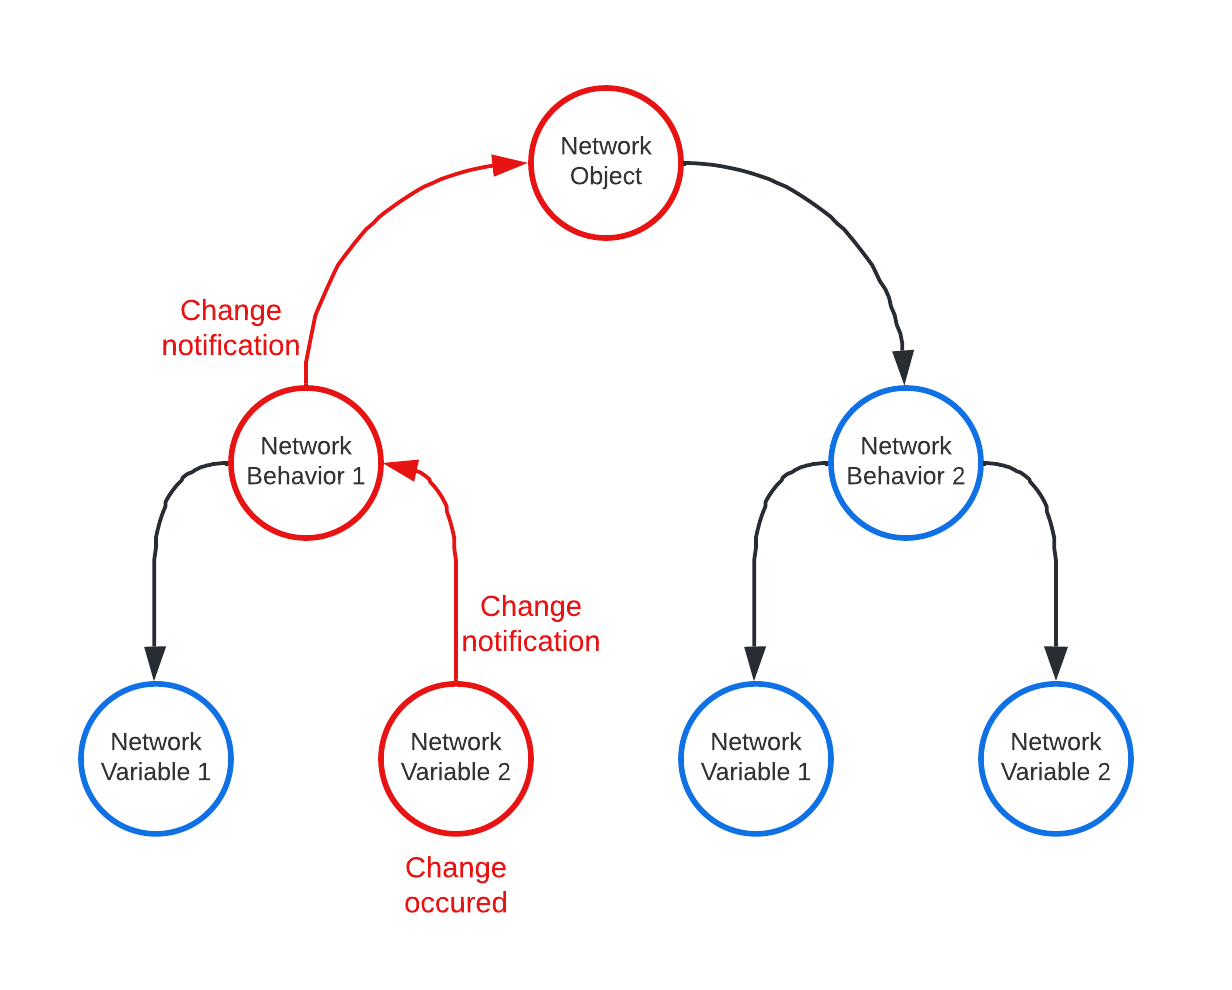
\includegraphics[scale=0.3]{NetworkObject-propagation-of-change}
	\caption{Propagation of change through the hierarchy (red color represents modified/dirty node) - single NetworkVariable change is going to mark parent NetworkBehavior as dirty, as well as grandparent NetworkObject node.}
	\label{fig:network-object-propagation}
\end{figure}

Even though this system outputs which networked objects have been modified, we still need a way to efficiently broadcast the changes so other process instances can update their local version of the state. Such system needs to broadcast only those variables that have been changed, as broadcasting whole state of an object each time a single variable changes would be extremely inefficient and bandwidth-wasteful.\\

To achieve such system, each NetworkObject and NetworkBehavior maintains a \textit{dirty bit-field} where each bit indicates whether a child node has been modified (\ref{fig:network-object-bit-field}). Order of bits corresponds to order of child nodes - first bit represents left-most child node, second bit node right next to it and so on. Bit-field is of fixed size (32 bits in the library) which imposes a limit on the number of child nodes a single node can have.

\begin{figure}[H]
	\centering
	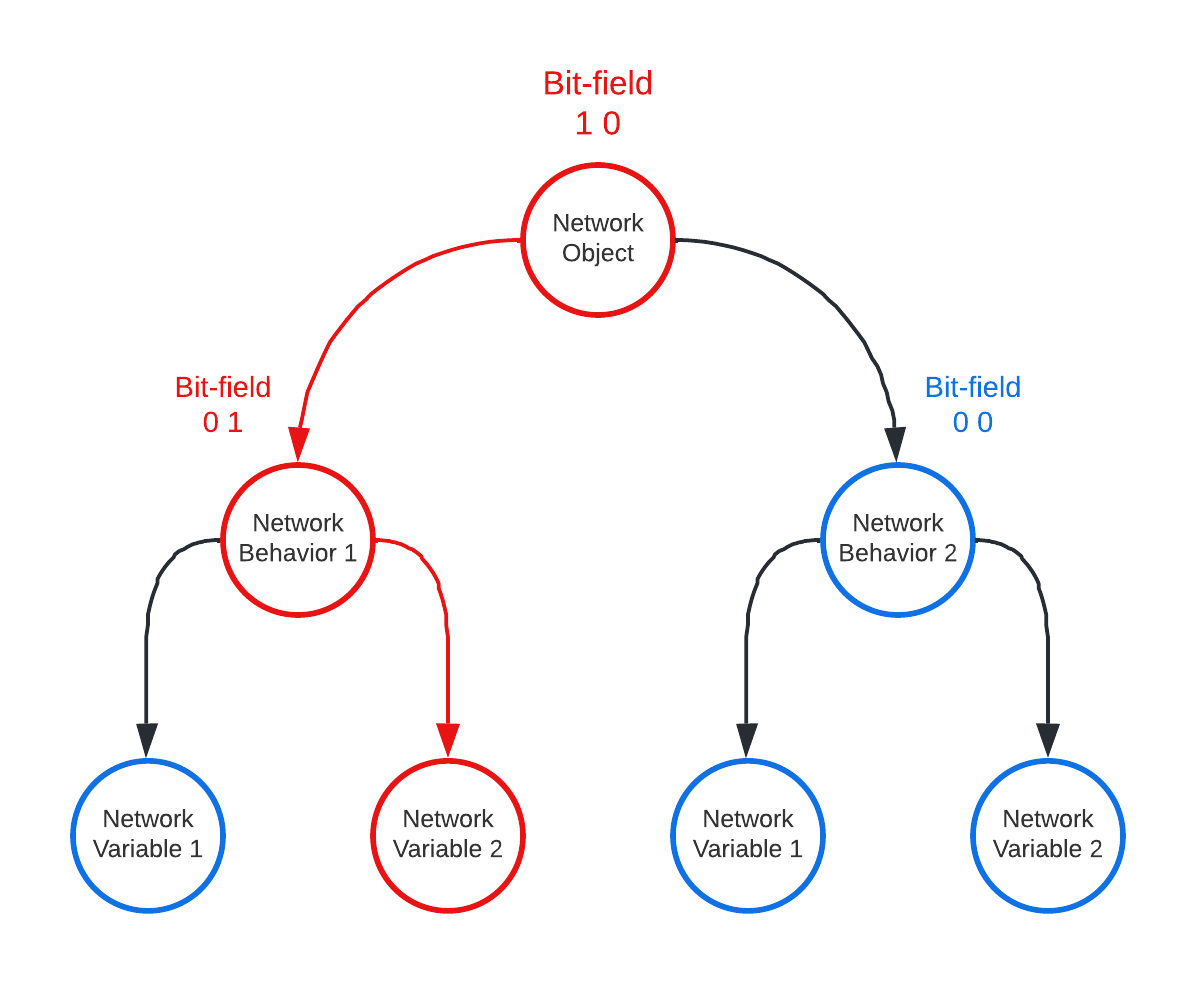
\includegraphics[scale=0.3]{NetworkObject-bit-field}
	\caption{Values of dirty bit-fields - root node has two child behavior nodes and only left child is dirty, so left bit is set to 1 and right bit is 0. Using exact same logic, left behavior has dirty bit-field of 01 as only right variable is modified, while right behavior has 00 bit-field as no variables have been modified.}
	\label{fig:network-object-bit-field}
\end{figure}

\begin{algorithm}[H]
	\caption{Encoding state synchronization packet}
	\textbf{Input:} Dirty NetworkObject node \\
	\textbf{Output:} Packet containing only modified state variables \\
	
	\begin{algorithmic}
		\State $packet \gets empty \; reliable \; packet$
		\State $packet \gets object.id$
		\State $packet \gets object.dirtyBitField$
		\State
		
		\ForEach {$behavior \in object.dirtyBehaviors $}
			\State $packet \gets behaviour.dirtyBitField$
			\State
			
			\ForEach {$variable \in behavior.dirtyVariables $}
				\State $packet \gets variable$
			\EndFor
			
			\State
			\State $behaviour.dirtyBitField = 0$
		\EndFor
		
		\State
		\State $object.dirtyBitField = 0$
		\State \Return $packet$
	\end{algorithmic}
\end{algorithm}

With such system, we can easily encode and transmit only changed nodes and receiver can just as easily receive, decode and update its local state.

\subsection{Remote procedure calls (RPCs)}
Remote procedure call\footnote{https://en.wikipedia.org/wiki/Remote\_procedure\_call} (RPC) is a mechanism for executing a piece of code on the remote machine. High-level library supports two types of RPCs: server RPC and client RPC. Server RPC is a method that is called on the client, but executed on the server, while client RPC is called on the server but executed on the client (\ref{fig:rpc-diagram}).

\begin{figure}[H]
	\centering
	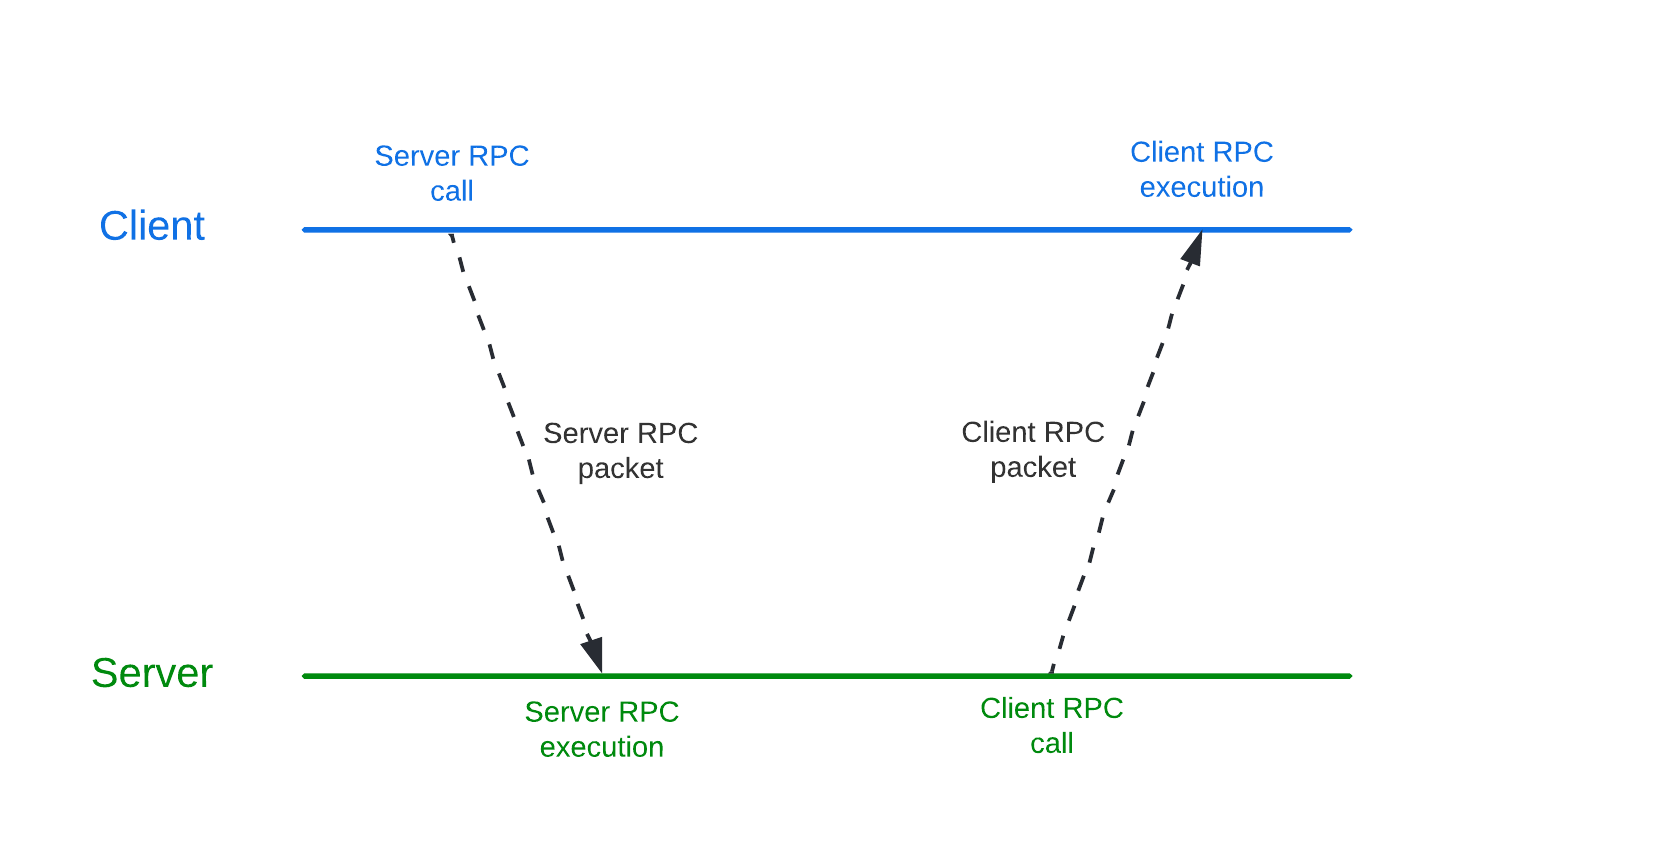
\includegraphics[scale=0.25]{NetworkBehavior-RPC-diagram}
	\caption{Diagram that shows how RPC works. In case of server RPC, client initiates the call by sending packet containing information required to execute the RPC. Once received by the server, actual method body is executed. Same logic applies to client RPC, with server calling and client executing.}
	\label{fig:rpc-diagram}
\end{figure}

As remote procedure calls are actual method calls, with only difference being the location of execution, they should also have the ability to accept method parameters. In order to understand how that is achieved, RPC packet (\ref{fig:rpc-packet-structure}) must be examined.

\begin{figure}[H]
	\centering
	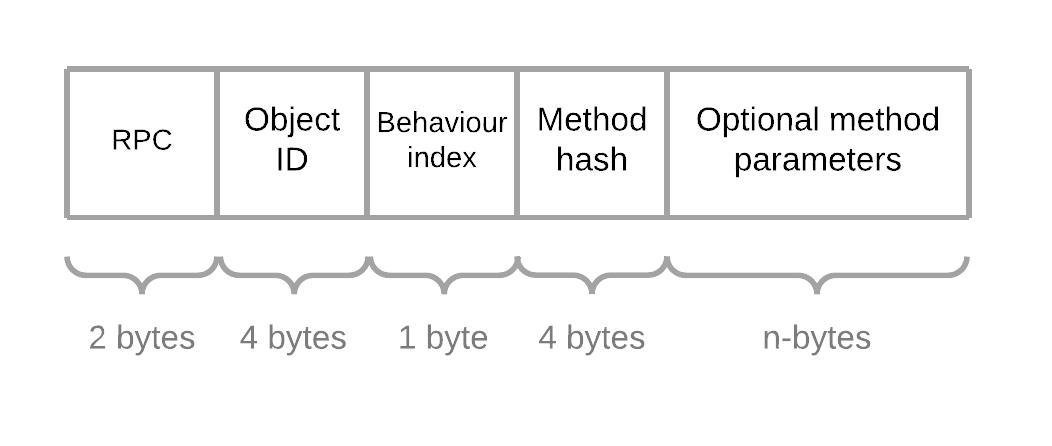
\includegraphics[scale=0.3]{NetworkBehavior-RPC-packet-structure}
	\caption{Structure of the RPC packet.}
	\label{fig:rpc-packet-structure}
\end{figure}

Packet starts with 2-bytes that indicate it is an RPC packet. It is followed by an object ID and behavior index that uniquely point to a specific NetworkBehavior which should execute the method call. After that hash is inserted that uniquely identifies a specific method (hash is calculated by hashing fully qualified method name and ensuring there are no hash conflicts). Finally, method parameters are inserted, if needed. With this information, receiver of the RPC packet can execute the method.

\section{Network Transform}
\textit{NetworkTransform} (\ref{fig:network-transform-inspector}) is a concrete implementation of \textit{NetworkBehavior} that solves the problem of synchronizing object's position (\ref{fig:network-transform-position-diagram}), rotation and scale.

\begin{figure}[H]
	\centering
	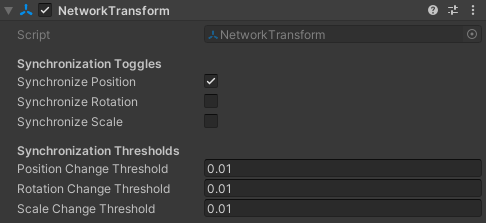
\includegraphics[scale=1.1]{NetworkTransform-inspector}
	\caption{NetworkTransform component displayed inside Unity's inspector.}
	\label{fig:network-transform-inspector}
\end{figure}

It is a powerful component that allows user to synchronize object's transform by simply attaching the component to it. Since transform synchronization is one of the most commonly encountered problems when creating a networked game, general solutions such as this one save developers a lot of time.\\

However, since transform synchronization is so common, simple ease of use is not enough; it also must be efficient. Component has to be able to support potentially hundreds of simultaneous instances and to achieve that it exploits the following facts:

\begin{enumerate}
	\item Object's rotation or scale is in many cases never-changing. That fact can be exploited to save bandwidth by giving the user ability to disable synchronization of particular transport's component (position, rotation or scale). If a component is disabled, its data is never going to be added to the outgoing synchronization packet, saving valuable bandwidth.
	
	\item If object's transform does not change, it does not need to be synced. Transform is marked as changed only if one of its enabled components' values has been changed by a value greater than threshold defined for that component. if transform is changed, only modified components are included in the sync packet. This way only changed components of changed transforms are synced, massively reducing the number of sync packets required.
\end{enumerate}

\begin{figure}[H]
	\centering
	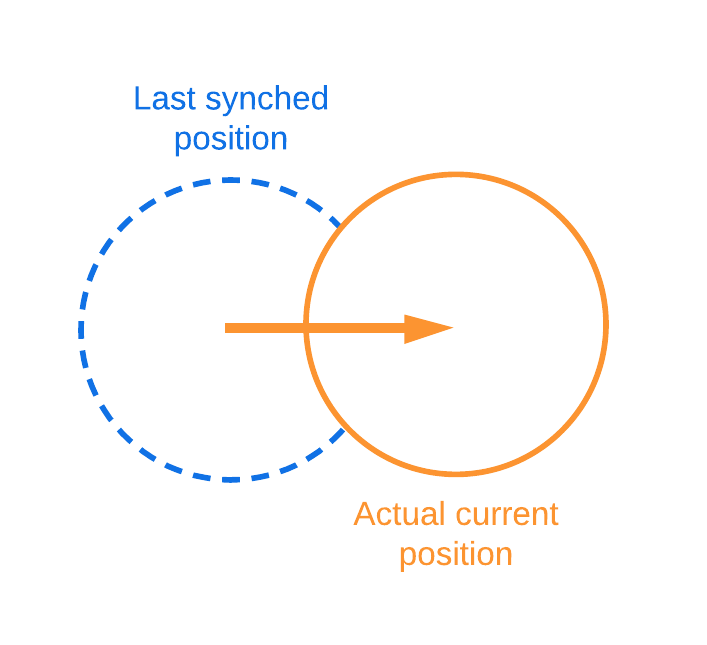
\includegraphics[scale=0.28]{NetworkTransform-position-diagram}
	\caption{Example of position synchronization. Orange arrow is a delta vector that shows the change in position since last synchronization. If length of the delta vector exceeds user-defined threshold, synchronization will occur.}
	\label{fig:network-transform-position-diagram}
\end{figure}

\textit{NetworkTransform} is also allowed on nested objects (for example, player's body could have one, but also player's head another, which synchronizes only head rotation). In order to understand how this is achieved, packet structure (\ref{fig:network-transform-packet-structure}) must be explained.

\begin{figure}[H]
	\centering
	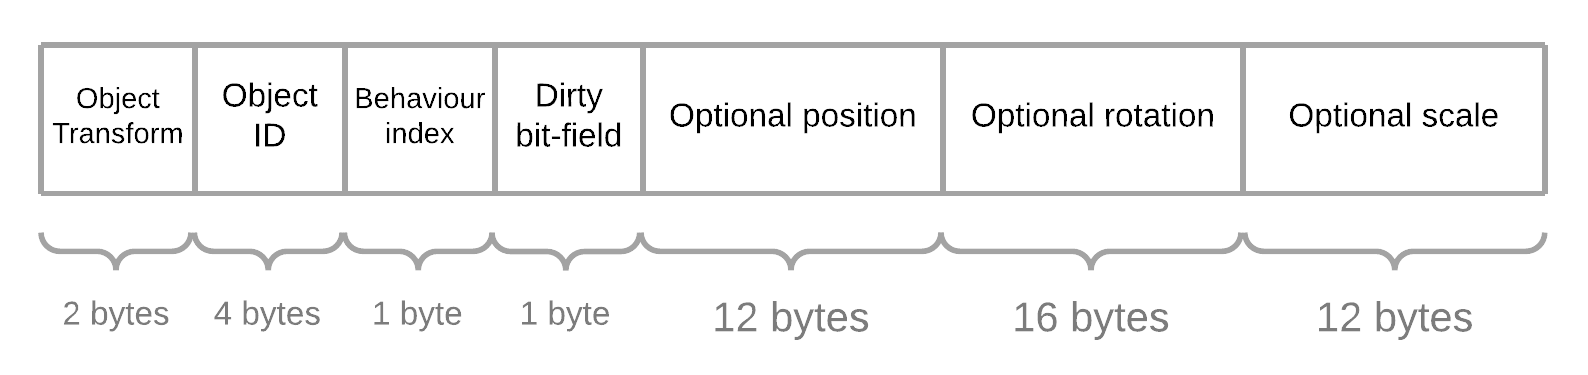
\includegraphics[scale=0.25]{NetworkTransform-packet-structure}
	\caption{Structure of the packet that is sent by the \textit{NetworkTransform} component.}
	\label{fig:network-transform-packet-structure}
\end{figure}

Component starts by inserting 2-byte value that indicates that packet contains object transform information. It is followed by specific object's ID that uniquely identifies it, allowing receiver to know which exactly which object's transform should be modified. After that, behavior index is provided to the receiver, which allows the receiver to know which exact child transform should be modified (this information allows for nested networked transforms).\\

To indicate whether a transform's component is included in a packet, so called \textit{dirty bit-field} is used. It is a single byte whose first bit indicates whether position is included in the packet, second bit indicates whether rotation is included and third bit indicates whether scale is included. In the end, actual position, rotation and/or scale of an object is provided.\\

This component uses sequenced channel to send its packets, as only the most recent data is relevant. This system provides user with a very simple, but bandwidth-efficient way to synchronize transform of any networked object. 

\section{Network Spawner}
\textit{NetworkSpawner} (\ref{fig:network-spawner-inspector}) is a concrete implementation of \textit{NetworkBehavior} that spawns and despawns objects when a client connects or disconnects from the server.

\begin{figure}[H]
	\centering
	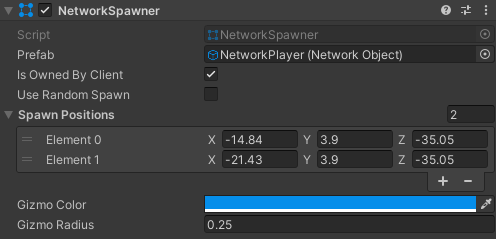
\includegraphics[scale=0.9]{NetworkSpawner-inspector}
	\caption{NetworkSpawner component displayed inside Unity's inspector.}
	\label{fig:network-spawner-inspector}
\end{figure}

\begin{table}[H]
	\centering
	\begin{tabular}{|c|c|}
		\hline
		\textbf{Field}     & \textbf{Description}                                                                                                       \\ \hline
		Prefab             & Defines which object should be spawned.                                                                                    \\ \hline
		Is Owned By Client & \begin{tabular}[c]{@{}c@{}}If true, ownership of the spawned object\\ will be given to the connecting client.\end{tabular} \\ \hline
		Use Random Spawn   & \begin{tabular}[c]{@{}c@{}}If true, position of the spawned object\\ will be chosen at random.\end{tabular}                \\ \hline
		Spawn Positions    & \begin{tabular}[c]{@{}c@{}}List of all the possible positions a newly\\ spawned object can be placed at.\end{tabular}      \\ \hline
		Gizmo Color        & \begin{tabular}[c]{@{}c@{}}Color of the sphere gizmo that shows\\ all of the spawn positions.\end{tabular}                 \\ \hline
		Gizmo Radius       & Radius of the gizmo sphere.                                                                                                \\ \hline
	\end{tabular}
	\caption{NetworkSpawner fields.}
	\label{table:network-spawner-fields}
\end{table}

It is a simple component that works in the following manner: whenever a new client is spawned, it firstly chooses a spawn position (\ref{table:network-spawner-gizmos}). If \textit{Use Random Spawn} option is selected, position will be chosen randomly from the \textit{Spawn Positions} list (otherwise, positions are chosen in order and wrap around when exhausted). \\

After spawn position has been selected, object defined by \textit{Prefab} field is spawned and all of the clients are informed about it. Finally, if \textit{Is Owned By Client} option is selected, ownership of the spawned object is given to the connecting client. \\

Component also keeps track of all the spawned objects so when a client disconnects it simply despawns object associated with the disconnecting client. This component is server-only, meaning it cannot run on a client.

\begin{figure}[H]
	\centering
	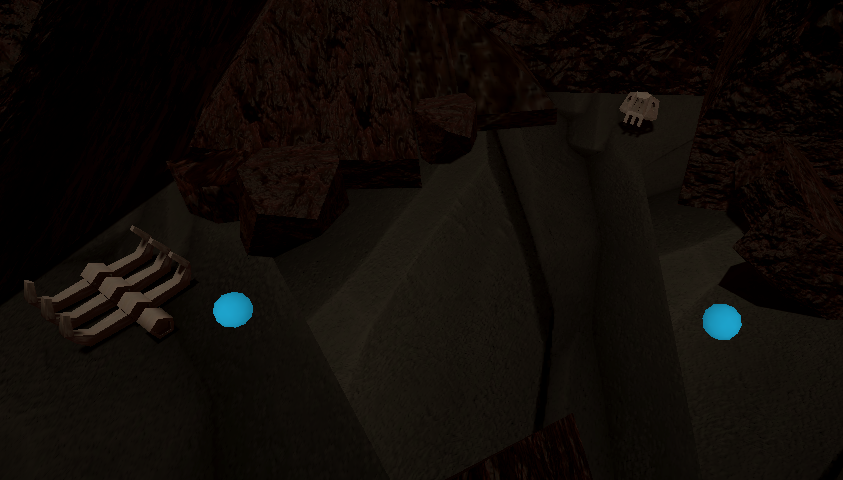
\includegraphics[scale=0.65]{NetworkSpawner-example}
	\caption{NetworkSpawner gizmos displayed inside Unity's scene view. Blue spheres give visual cue to where spawn positions are in placed in the world.}
	\label{table:network-spawner-gizmos}
\end{figure}

\chapter{Application}
This chapter showcases and explains the networking behind a multiplayer game that was build using previously described high-level networking library. The game was inspired by a classic title \textit{Doom}\footnote{https://en.wikipedia.org/wiki/Doom\_(1993\_video\_game)} in which player has to defeat waves of incoming enemies. The game consists of a game menu and a game scene.

\section{Game menu}
Upon entering the application, user is placed in the game menu (\ref{fig:main-menu}). It is a simple scene that allows the user to either create, join or exit the game.

\begin{figure}[H]
	\centering
	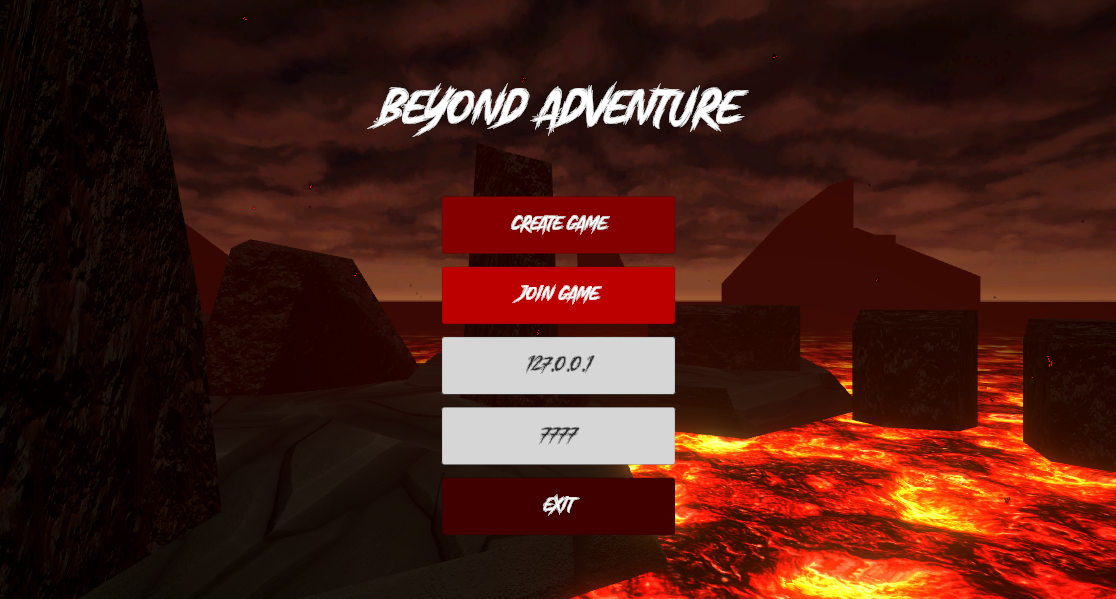
\includegraphics[scale=0.5]{MainMenu}
	\caption{View into the game menu.}
	\label{fig:main-menu}
\end{figure}

\textit{Create game} button turns the local application instance into a host which acts as both client and server. This means other players can join the game by connecting to the host's IP address and port combination (where port is determined by the second input field in the menu). \textit{Join game} button attempts to join an already existing game that was started by another application instance. Destination at which attempt will be made is determined by the first and second input fields - first input field represents IP address and second defines the port number. \textit{Exit} button terminates the application process.

\section{Game scene}
Once a game has been either created or joined, player is placed in the game scene. It has a dark atmosphere and consists of a rocky map surrounded by moving lava (\ref{fig:game-map}).\\

\begin{figure}[H]
	\centering
	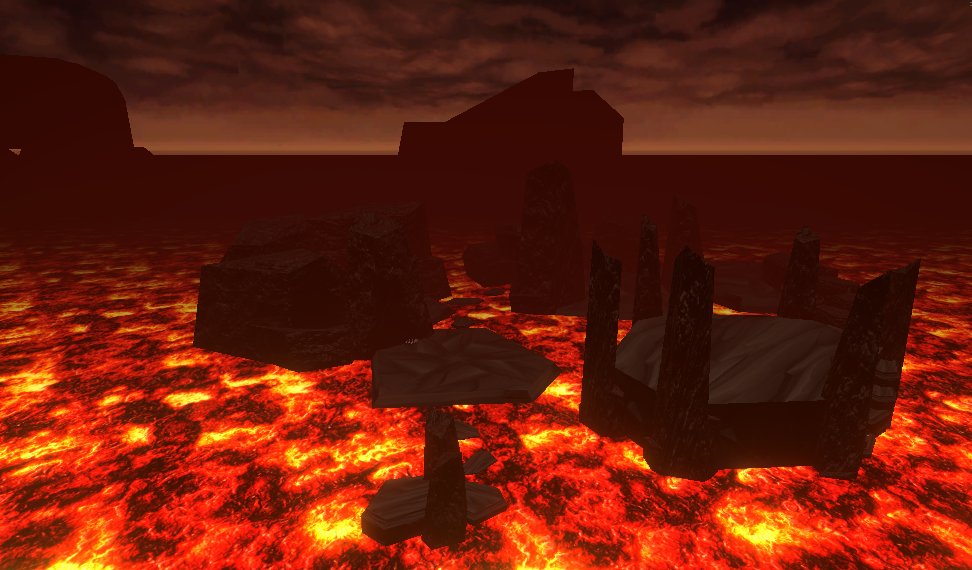
\includegraphics[scale=0.56]{Game-map}
	\caption{Map as seen from the bird's eye-view.}
	\label{fig:game-map}
\end{figure}

Main goal of the game is to defeat incoming enemy waves, which get progressively harder by having more enemies which also get stronger. To help player defeat enemy waves, gun is provided which can be used to shoot enemies from far away. However, gun has limited ammunition, so player has to keep moving around the map where more ammo can be found. \\

Player also has limited health which decreases with each enemy hit (\ref{fig:game-spawn}). If it reaches zero, player dies. If all the players die, game is finished and a new game must be created.

\begin{figure}[H]
	\centering
	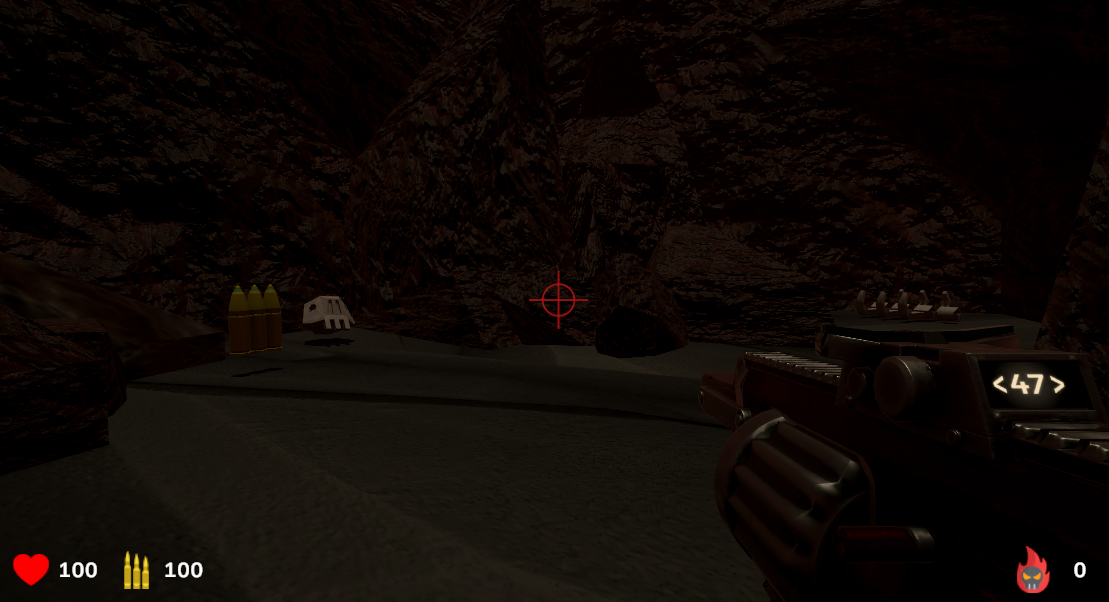
\includegraphics[scale=0.5]{Game-spawn}
	\caption{Game from the player's point of view. In the bottom left corner, player can always get information about current health and ammo. Bottom right corner displays number of enemies alive.}
	\label{fig:game-spawn}
\end{figure}

In order to help player survive and defeat enemy waves, various items called \textit{pick-ups} are scattered across the map (\ref{fig:game-pick-ups}). When those are picked-up, they grant player a useful resource.

\begin{figure}[H]
	\centering
	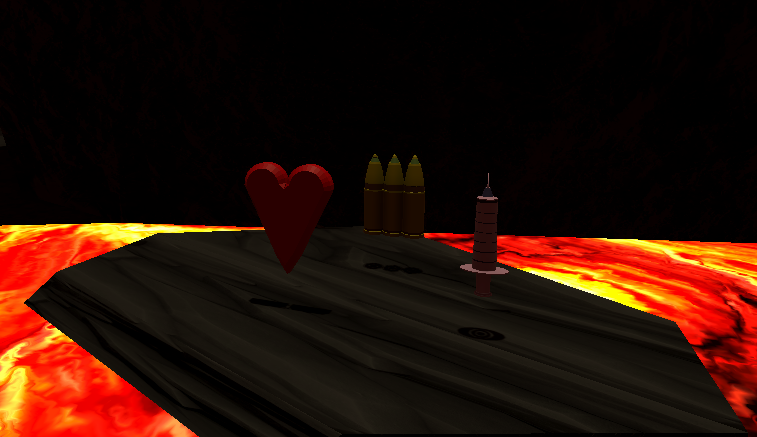
\includegraphics[scale=0.55]{Game-pick-ups}
	\caption{Example of pick-ups that can be found on the map. There are three types: health and ammo pick-ups which restores some of the player's health and ammo respectively, and steroid which grants player the ability to perform big jumps for a certain period of time.}
	\label{fig:game-pick-ups}
\end{figure}

\subsection{Networking implementation}
This section is going to explain how multiplayer was implemented in the game scene by utilizing the high-level library.\\

For initial spawning of the players that join the game (\ref{fig:game-players-at-spawn}), \textbf{NetworkSpawner} component is used. It simply spawns a prefab of the player on a predefined position once it successfully joins the game.\\

\begin{figure}[H]
	\centering
	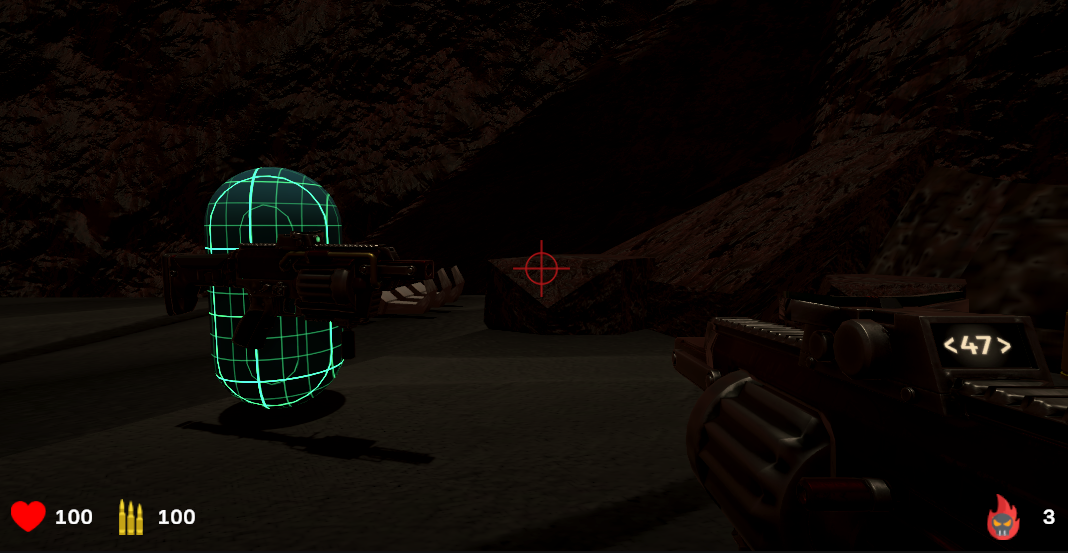
\includegraphics[scale=0.5]{Game-players-at-spawn}
	\caption{Players that have joined the game and were placed on their spawn positions.}
	\label{fig:game-players-at-spawn}
\end{figure}

After a player has joined, wave spawning logic will start. That logic is executed exclusively by the server in order to ensure server-authority. It includes spawning of enemies via \textbf{NetworkManager} and tracking when new ones should be spawned. It consists of multiple spawn actions, where each action spawns certain amount of enemies in a specific predefined spawn area (\ref{fig:game-spawn-areas}).\\

\begin{figure}[H]
	\centering
	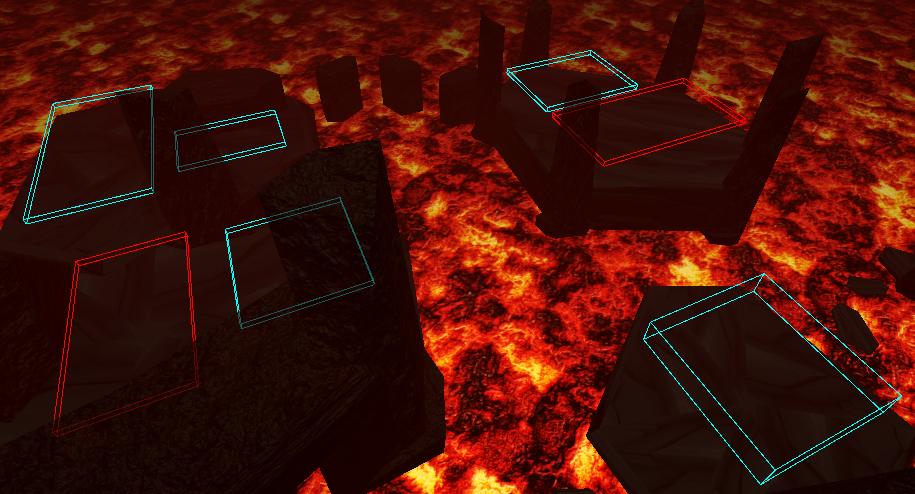
\includegraphics[scale=0.58]{Game-spawn-areas}
	\caption{All of the defined spawn areas which are used by the wave spawning logic.}
	\label{fig:game-spawn-areas}
\end{figure}

Once first set of enemies has been spawned, game officially starts. Enemy behavior is controlled exclusively by the server using custom \textbf{NetworkBehavior} implementations. Their position, rotation and positions of bullets they shoot are all synchronized with a \textbf{NetworkTransform} component (\ref{fig:game-enemies-networked}).\\

\begin{figure}[H]
	\centering
	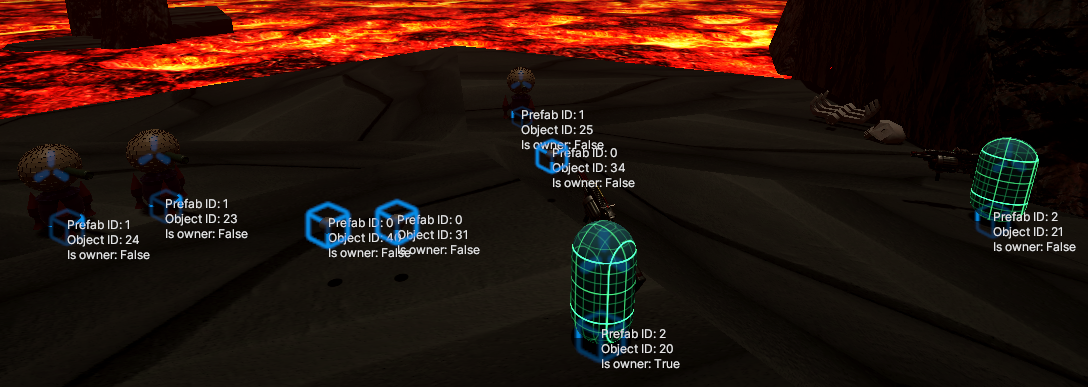
\includegraphics[scale=0.5]{Game-enemies-networked}
	\caption{View of the scene in the middle of combat. It consists of three enemy jet-pack riders (object IDs 23, 24 and 25) which are shooting bullets (IDs 31, 34 and 40) at two players that are in the game (IDs 20 and 21).}
	\label{fig:game-enemies-networked}
\end{figure}

Each pick-up in the game is also a networked object whose collision with the player is tracked by the server (this logic is encapsulated inside a custom \textbf{NetworkBehavior} implementation). Once a collision is detected, pick-up is disabled over the network and effect is applied to the player that triggered the collision (\ref{fig:game-pick-ups-networked}).

\begin{figure}[H]
	\centering
	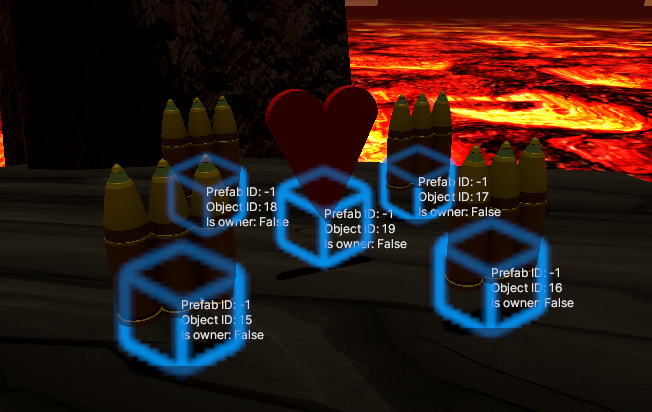
\includegraphics[scale=0.85]{Game-pick-ups-networked}
	\caption{Networked pick-ups in the game.}
	\label{fig:game-pick-ups-networked}
\end{figure}

If all players have been killed by the enemies, game is over and host of the game can either restart the game by pressing the \textit{Retry} button or can terminate the game session by pressing the \textit{Exit} button (\ref{fig:game-over}). Restarting the game causes a scene-reload on all clients and game logic is executed from start as described previously.

\begin{figure}[H]
	\centering
	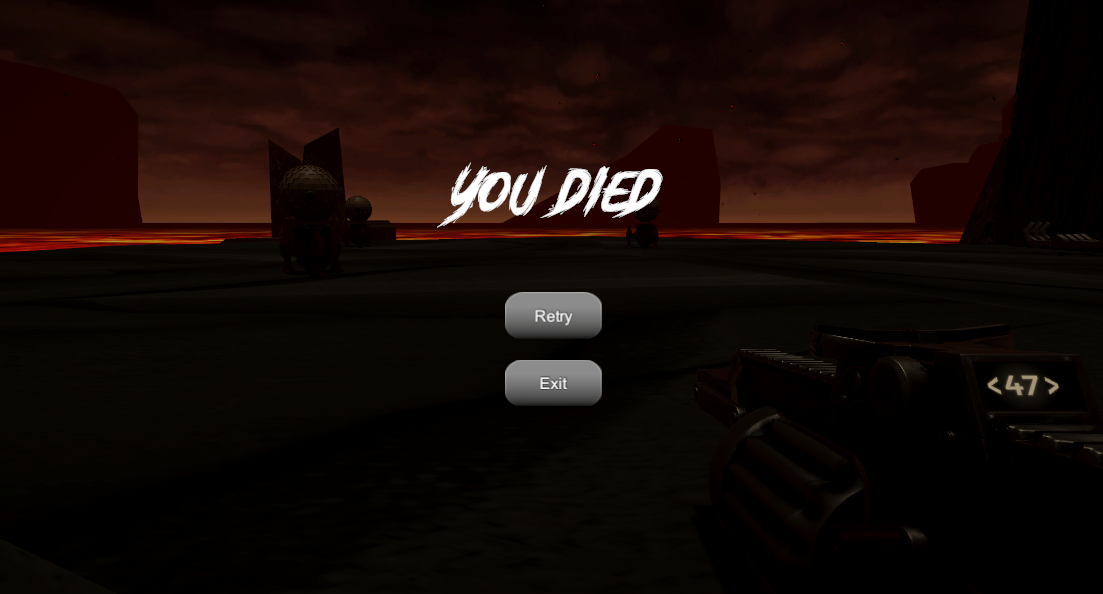
\includegraphics[scale=0.5]{Game-over}
	\caption{Game-over screen shown to the host once all players have been killed.}
	\label{fig:game-over}
\end{figure}



\subsection{Networking scripts}
This section lists and gives a brief explanation of all the scripts that have been developed to achieve multiplayer functionality in the game scene.

\begin{table}[H]
	\centering
	\resizebox{\columnwidth}{!}{%
		\begin{tabular}{|c|c|}
			\hline
			\textbf{Script Name}    & \textbf{Description}                                                        \\ \hline
			Lava                    & Moves lava up and down and deals damage to any player that touches it.      \\ \hline
			Enemy &
			\begin{tabular}[c]{@{}c@{}}Abstract base class of all the enemies in the game. Contains\\ enemy health and raises event when enemy is killed.\end{tabular} \\ \hline
			Jetpack Enemy Entity    & Defines collision logic with the player's bullet.                           \\ \hline
			Jetpack Enemy System    & Controls the movement and behavior of all the active jetpack enemies.       \\ \hline
			Turret Pod Enemy Entity & Defines collision logic with the player's bullet.                           \\ \hline
			Turret Pod Enemy System & Controls the movement and behavior of all the active turret pod enemies.    \\ \hline
			Bullet Entity           & Defines collision logic of a bullet.                                        \\ \hline
			Bullet System           & Controls the movement of all active bullets in the game scene.              \\ \hline
			Pick Up &
			\begin{tabular}[c]{@{}c@{}}Abstract base class of all the pick-ups in the game. Defines abstract\\ method for what should happen when on collision with a player.\end{tabular} \\ \hline
			Ammo Pick Up            & Increases player's ammo on collision.                                       \\ \hline
			Health Pick Up          & Increases player's health on collision.                                     \\ \hline
			Steroid Pick Up         & Increases player's jump height on collision (for a certain amount of time). \\ \hline
			Pick Up Respawn System  & Controls respawning of all pick-ups in the game scene.                      \\ \hline
			Wave Manager            & Performs the logic of spawning enemy waves.                                 \\ \hline
			Input State             & Synchronizes player's input with the server.                                \\ \hline
			Player Controller       & Contains and manages player's current state (ammo, health and jump height). \\ \hline
			Player Manager          & Keeps track of all the active players.                                      \\ \hline
			Gun Controller          & Controls player's shooting logic.                                           \\ \hline
			Network Object Pool     & Contains reuse logic of networked objects that are frequently used.         \\ \hline
		\end{tabular}%
	}
	\caption{All of the developed scripts used to implement multiplayer functionality.}
	\label{table:game-scene-network-scripts}
\end{table}



\chapter{Conclusion}
This thesis documents and explains the theory, implementation and application of a networking library designed for developing multiplayer games. Thesis consists of three main chapters, each documenting a single layer in the stack. Those chapters are:

\begin{enumerate}
	\item Transport chapter which describes an implementation of a low-level reliable UDP library.
	\item High-level chapter which describes Unity specific components that create powerful abstractions and allow users to easily develop complex networking solutions.
	\item Application chapter that showcases a game developed using high-level library. 
\end{enumerate}

Thesis also demonstrates that creating a multiplayer game is not an easy task and utilizing an existing networking solution is recommended. Finally, it provides detailed information about how a custom networking solution has been achieved in order to allow the reader to recreate such system for their own uses, if needed.

\bibliography{literature}
\bibliographystyle{fer}
\clearpage

\engtitle{Development and application of a videogame multiplayer networking library}
\begin{abstract}
This thesis documents and explains the theory, implementation and application of a networking library designed for developing multiplayer games.
	
\keywords{Networking, multiplayer, video-game, library}
\end{abstract}



\begin{sazetak}
Ovaj rad dokumentira i opisuje teoriju, implementaciju i primjenu knjižnice namjenjene za umrežavanje višekorisničkih videoigara.

\kljucnerijeci{Umrežavanje, višekorisnička, video-igra, knjižnica}
\end{sazetak}

\end{document}
